\section{Calibration before the installation in ProtoDUNE-SP}
\label{sec:old_calib}

\noindent The Lake Shore Cryotronics company provides PT102 RTDs with a temperature accuracy of about 0.1 K, which is insufficient for ProtoDUNE-SP's requirements. While the company offers additional calibration to the 10 mK level, the cost is prohibitive. R\&D on sensor calibration was identified as a crucial ingredient for the success of the ProtoDUNE-SP temperature monitoring system. For this particular application, sensor calibration consists in finding the temperature offset between any pair of sensors when exposing them to the same temperature. The experimental setup used for the calibration of RTDs before their installation in ProtoDUNE-SP had two main components: i) the readout system used to monitor the sensor's temperature (described in the previous section) and ii) the cryogenics vessel and the associated mechanical elements used to put sensors together under stable and homogeneous cryogenics conditions. They were developed to achieve a relative calibration with a precision better than 5 mK. %They are described in detail below.

%--------------------------------------------
\subsection{Experimental setup}
\noindent The mechanics of the calibration setup evolved significantly from the initial tests to the final Static TGM  calibration campaign. This evolution was primarily driven by the need to improve offset stability and repeatability. The final configuration (see Fig. \ref{fig:setup_final}) consisted of the following components:

\begin{itemize}
    \item A polystyrene vessel formed by an outer box with dimensions $35\times35\times30$ cm$^3$ and 4.5 cm thick walls, and a dedicated polystyrene cover, complemented by extruded polystyrene panels glued into the inner walls and floor of the outer box, to conform an inner empty volume of $10\times10\times20$ cm$^3$.
    \item A $10\times10\times20$ cm$^3$ 3D printed polylatic acid (PLA) box with two independent concentric volumes, placed in the inner volume of the polystyrene vessel. Its purpose is twofold: i) to contain LAr, since polystyrene is porous to it, and ii) to create an smaller inner volume  with further insulation and less convection.
    \item A cylindrical aluminum capsule, to be placed in the inner volume of the PLA box,  with 5 cm diameter, 12 cm height and 1 mm thin walls. It had a circular aluminum cover with a small opening to extract the cables and to allow LAr to penetrate inside. The capsule was used to slowly bring sensors to cryogenic temperatures by partial immersion in LAr with no liquid inside, minimizing thermal stress. Aluminum was chosen for its high thermal conductivity.
    \item  A 3D printed PLA support for four sensors, to be placed inside the aluminum capsule, keeping sensors always in the same position with respect to each other and to the capsule walls.
\end{itemize}

The system described above ensures sufficiently stable and homogeneous conditions within the inner volume, with three levels of insulation: the outer polystyrene vessel and two PLA box LAr volumes. The aluminium capsule is key to this system and its usage constituted a turning point in the R\&D since it minimises thermal shocks, which were identified as the main limiting factor for the repeatability of the sensor's offsets. Indeed, variations of several tenths of mK were observed during initial tests without the capsule. The problem was attributed to thermal shocks when, after many immersions in LN$_{2}$, one of the sensors suffered a dramatic change in its offset (see Fig.~\ref{fig:broken_sensor_evolution}). Examination at the microscope revealed cracks in the outer RTD ceramics (see Fig.~\ref{fig:broken_sensor}).

\begin{figure}[htbp]
\centering
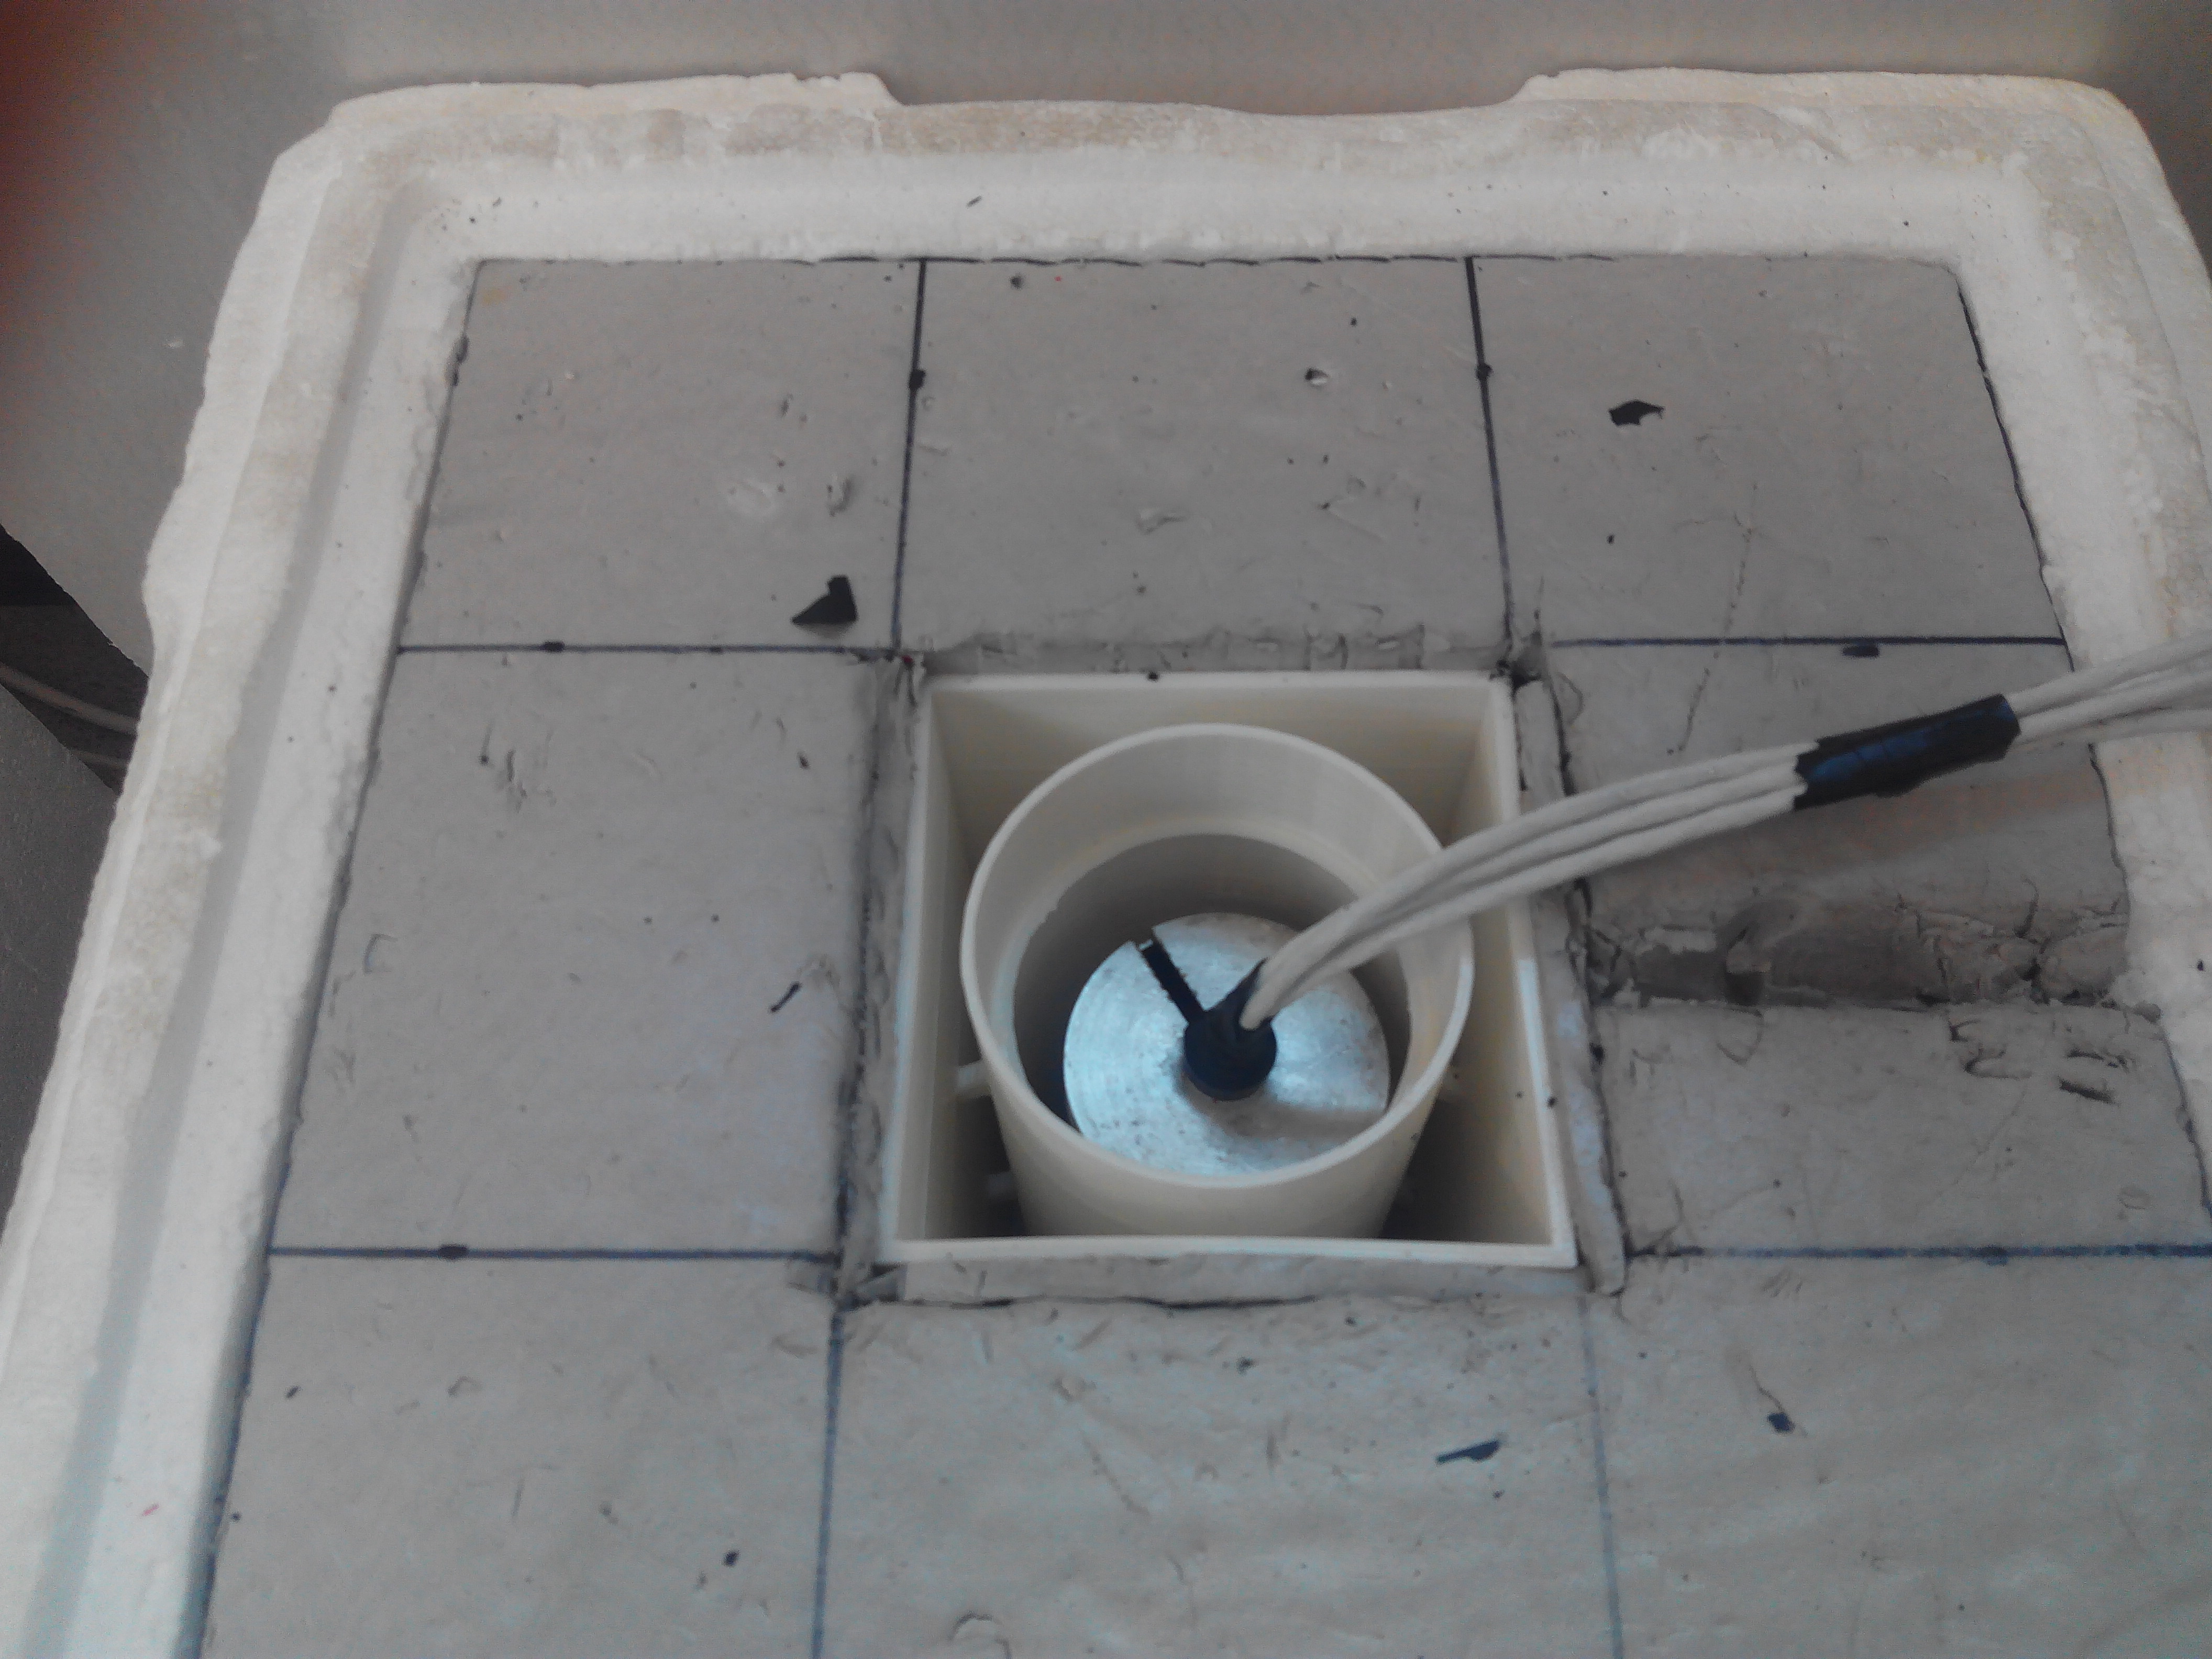
\includegraphics[width=0.32\textwidth]{images/figure_4_a.jpg}
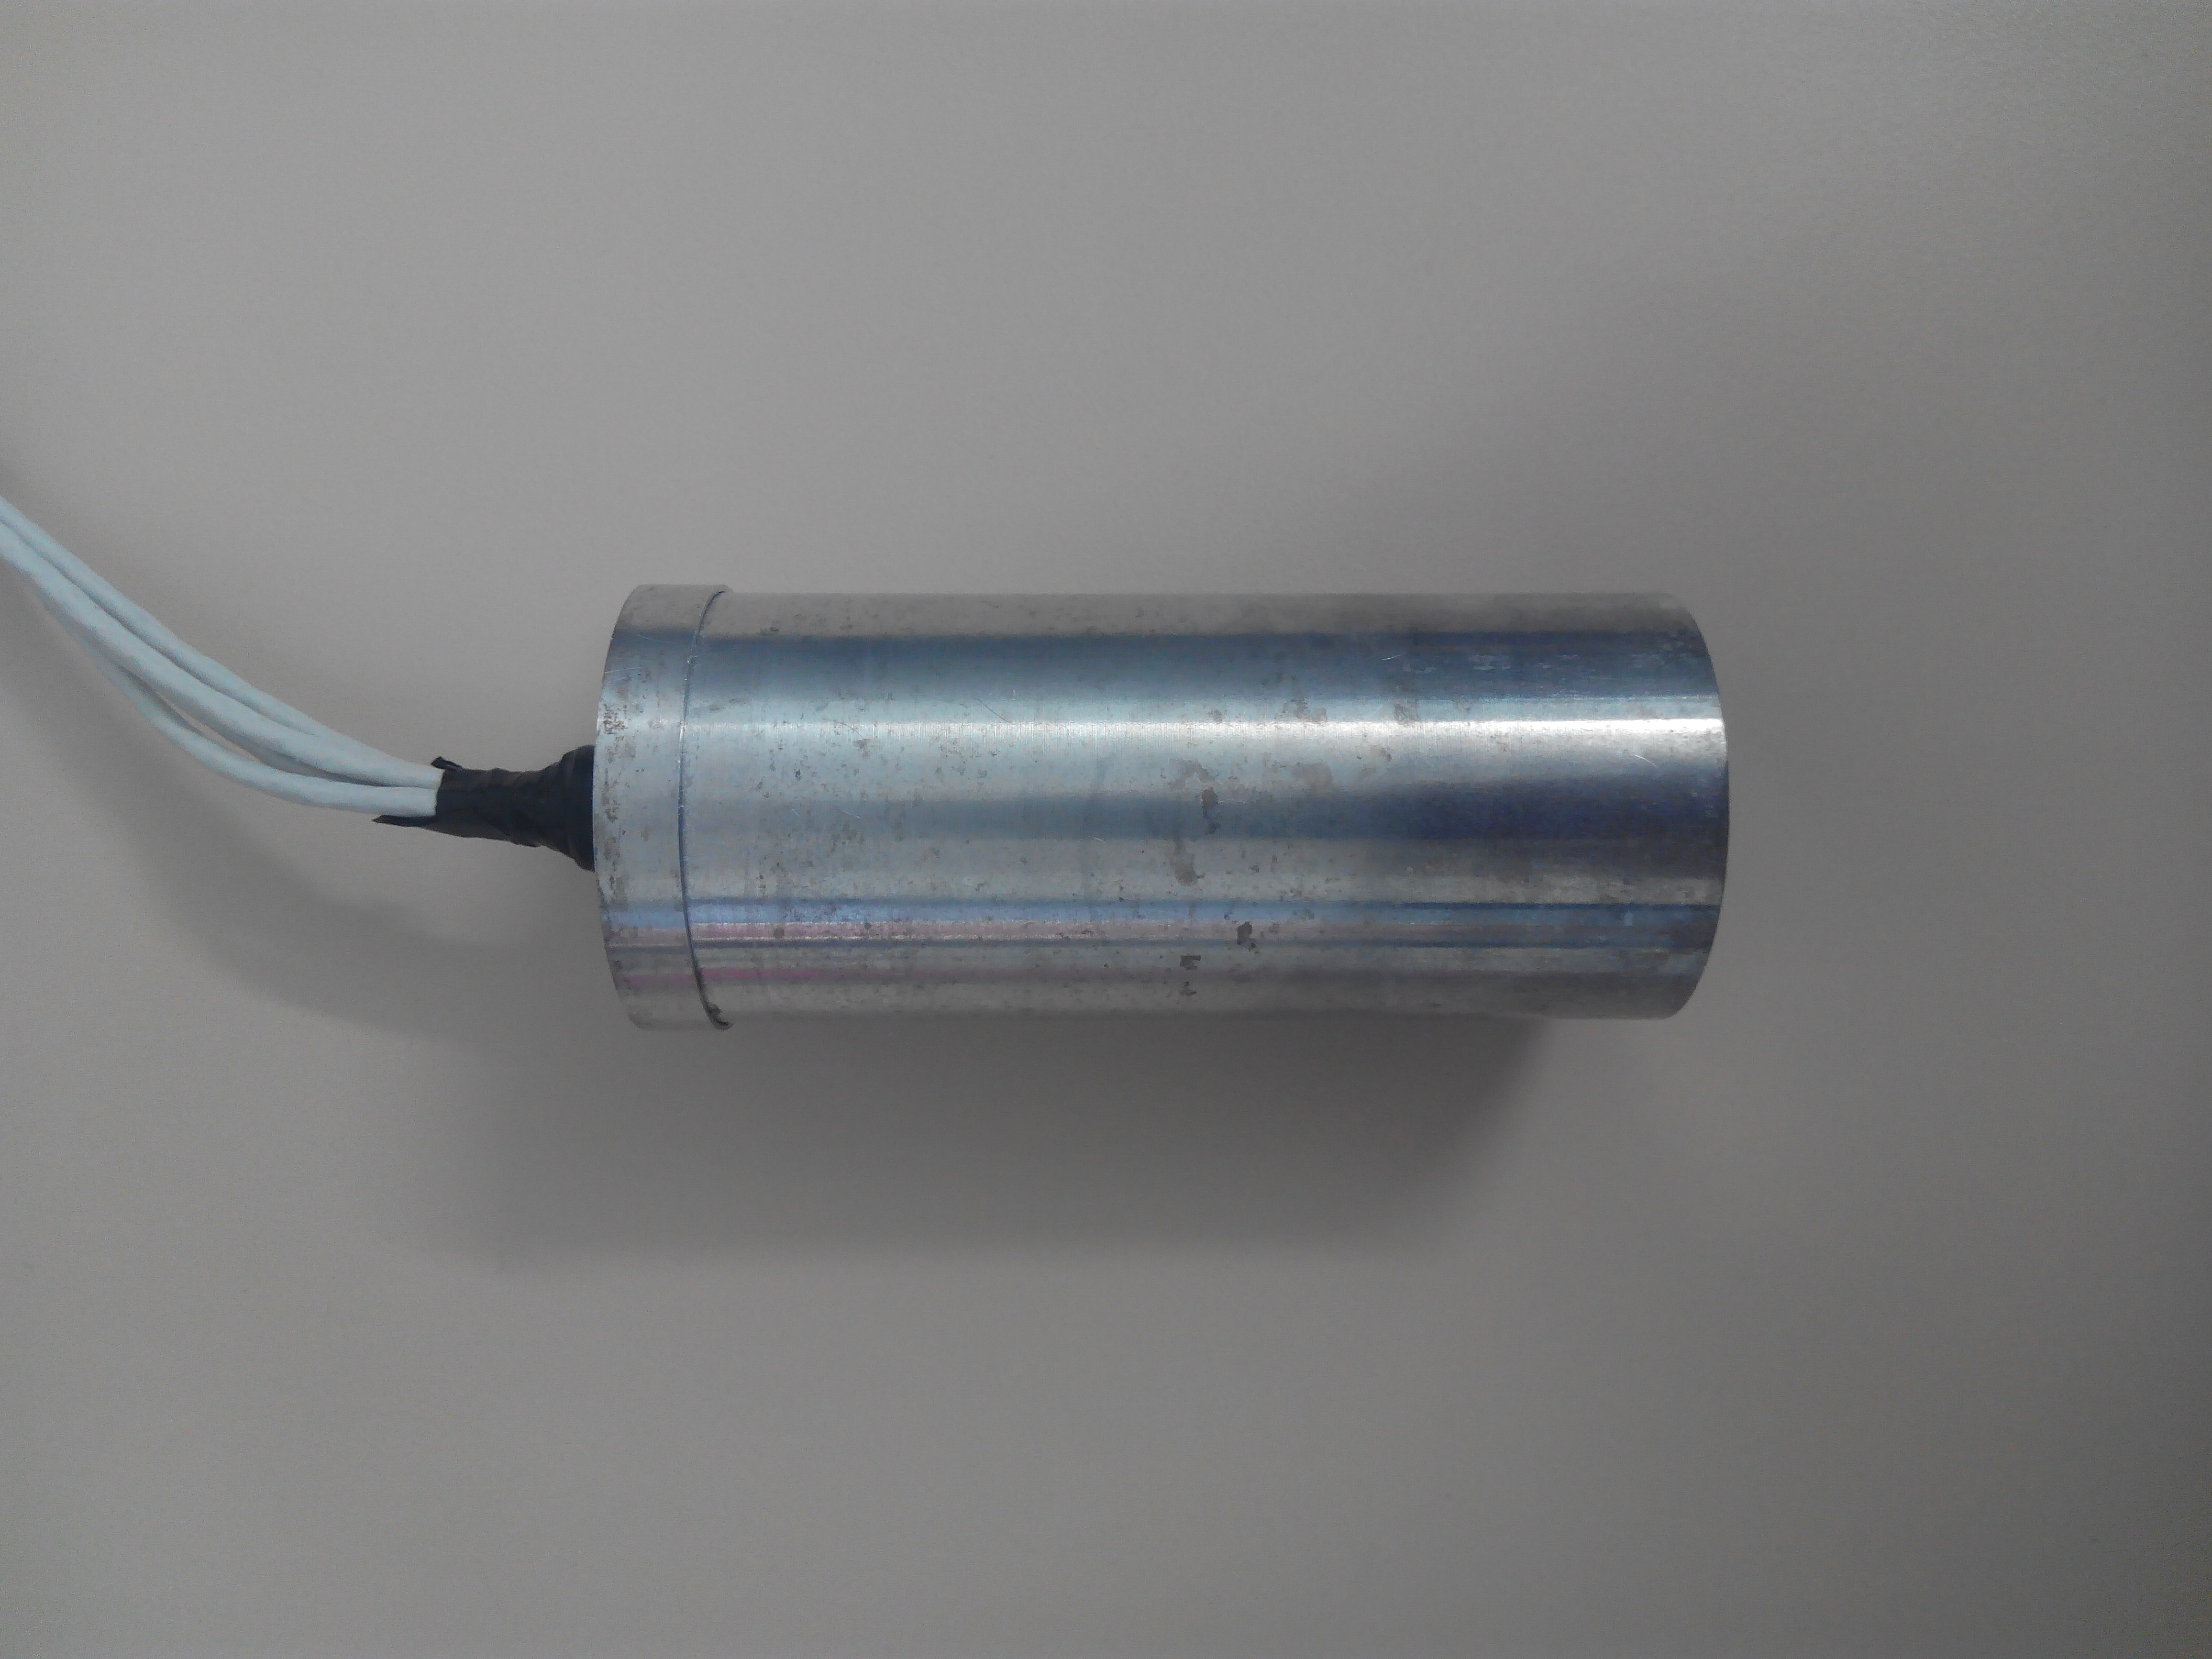
\includegraphics[width=0.32\textwidth]{images/figure_4_b.jpg}
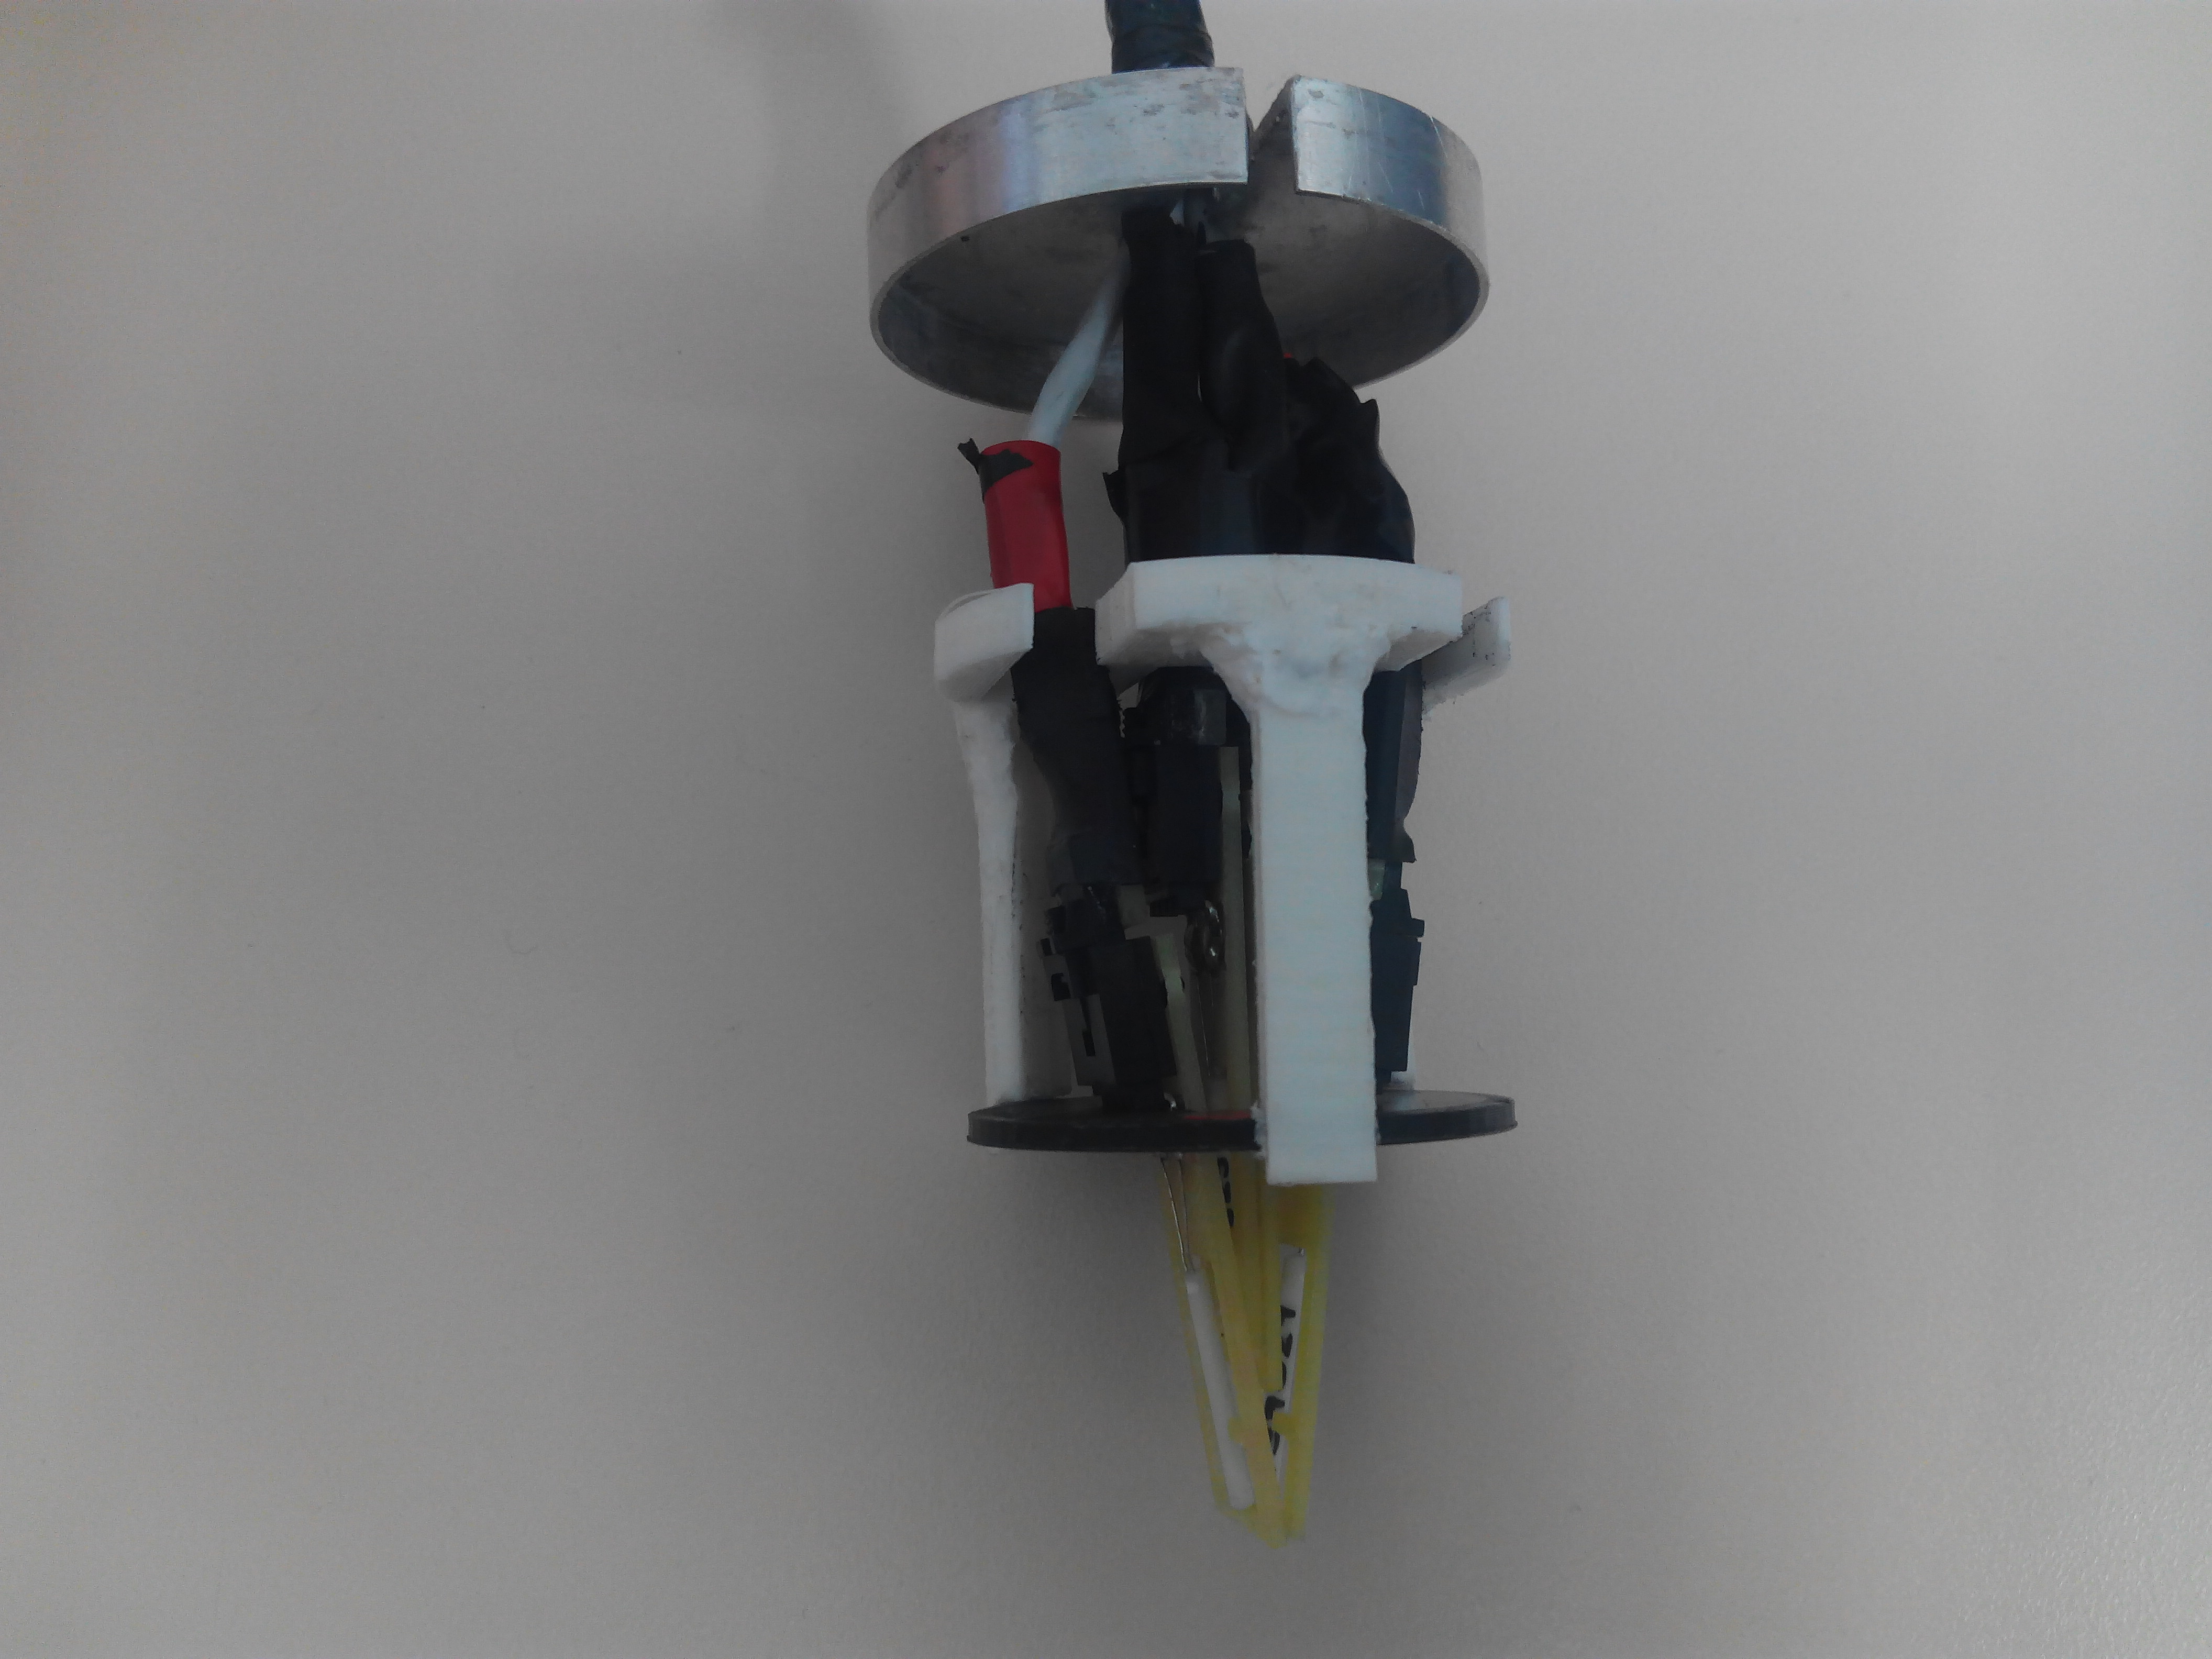
\includegraphics[width=0.32\textwidth]{images/figure_4_c.jpg}
\caption{Final calibration setup. Left: polystyrene box with PLA box and aluminum capsule. Middle: aluminum capsule. Right: Sensor's support with four sensors.
\label{fig:setup_final}}
\end{figure}

\begin{figure}[htbp]
\centering
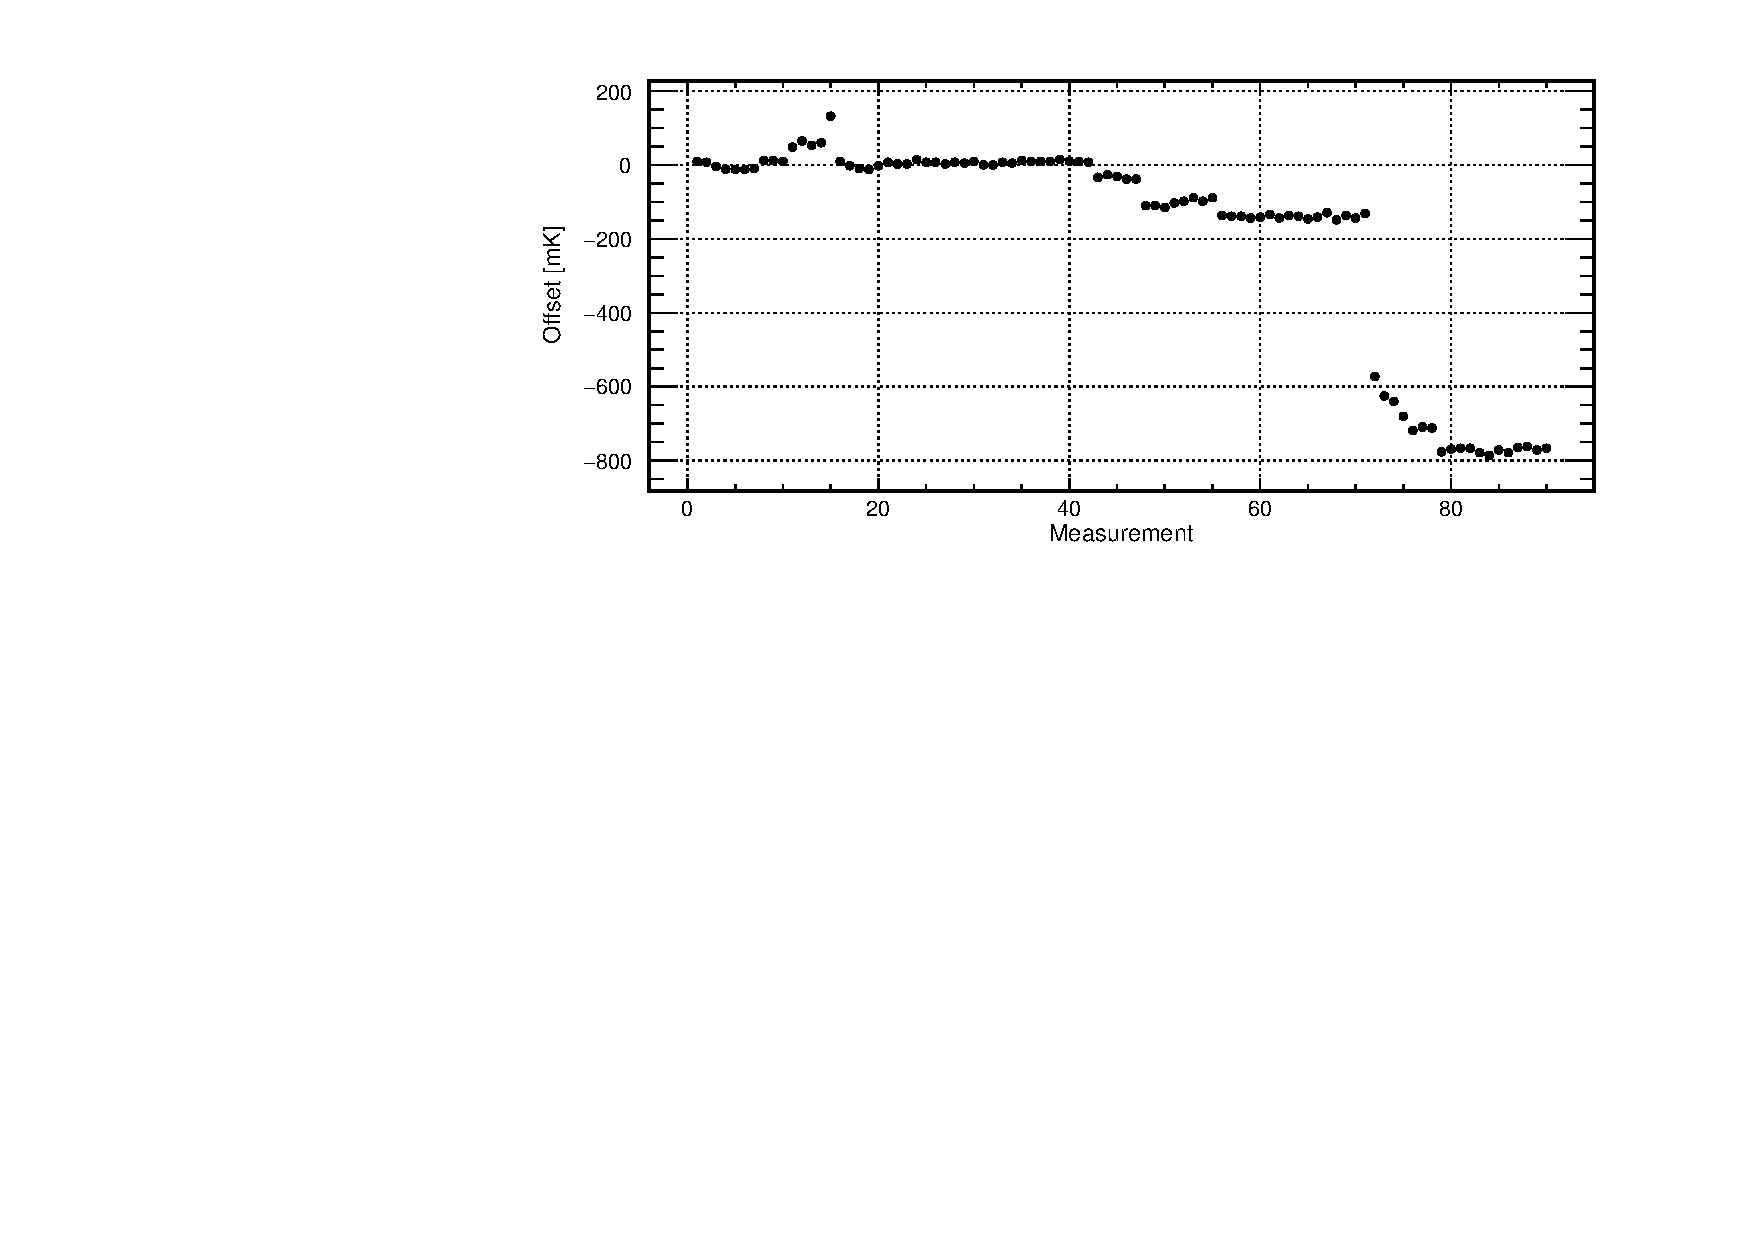
\includegraphics[width=0.9\textwidth]{images/figure_5.pdf}
\caption{Offset between two sensors for 90 immersions in LN2. A temperature drop of approximately 800 mK is observed around the 70th immersion point.
\label{fig:broken_sensor_evolution}}
\end{figure}

\begin{figure}[htbp]
\centering
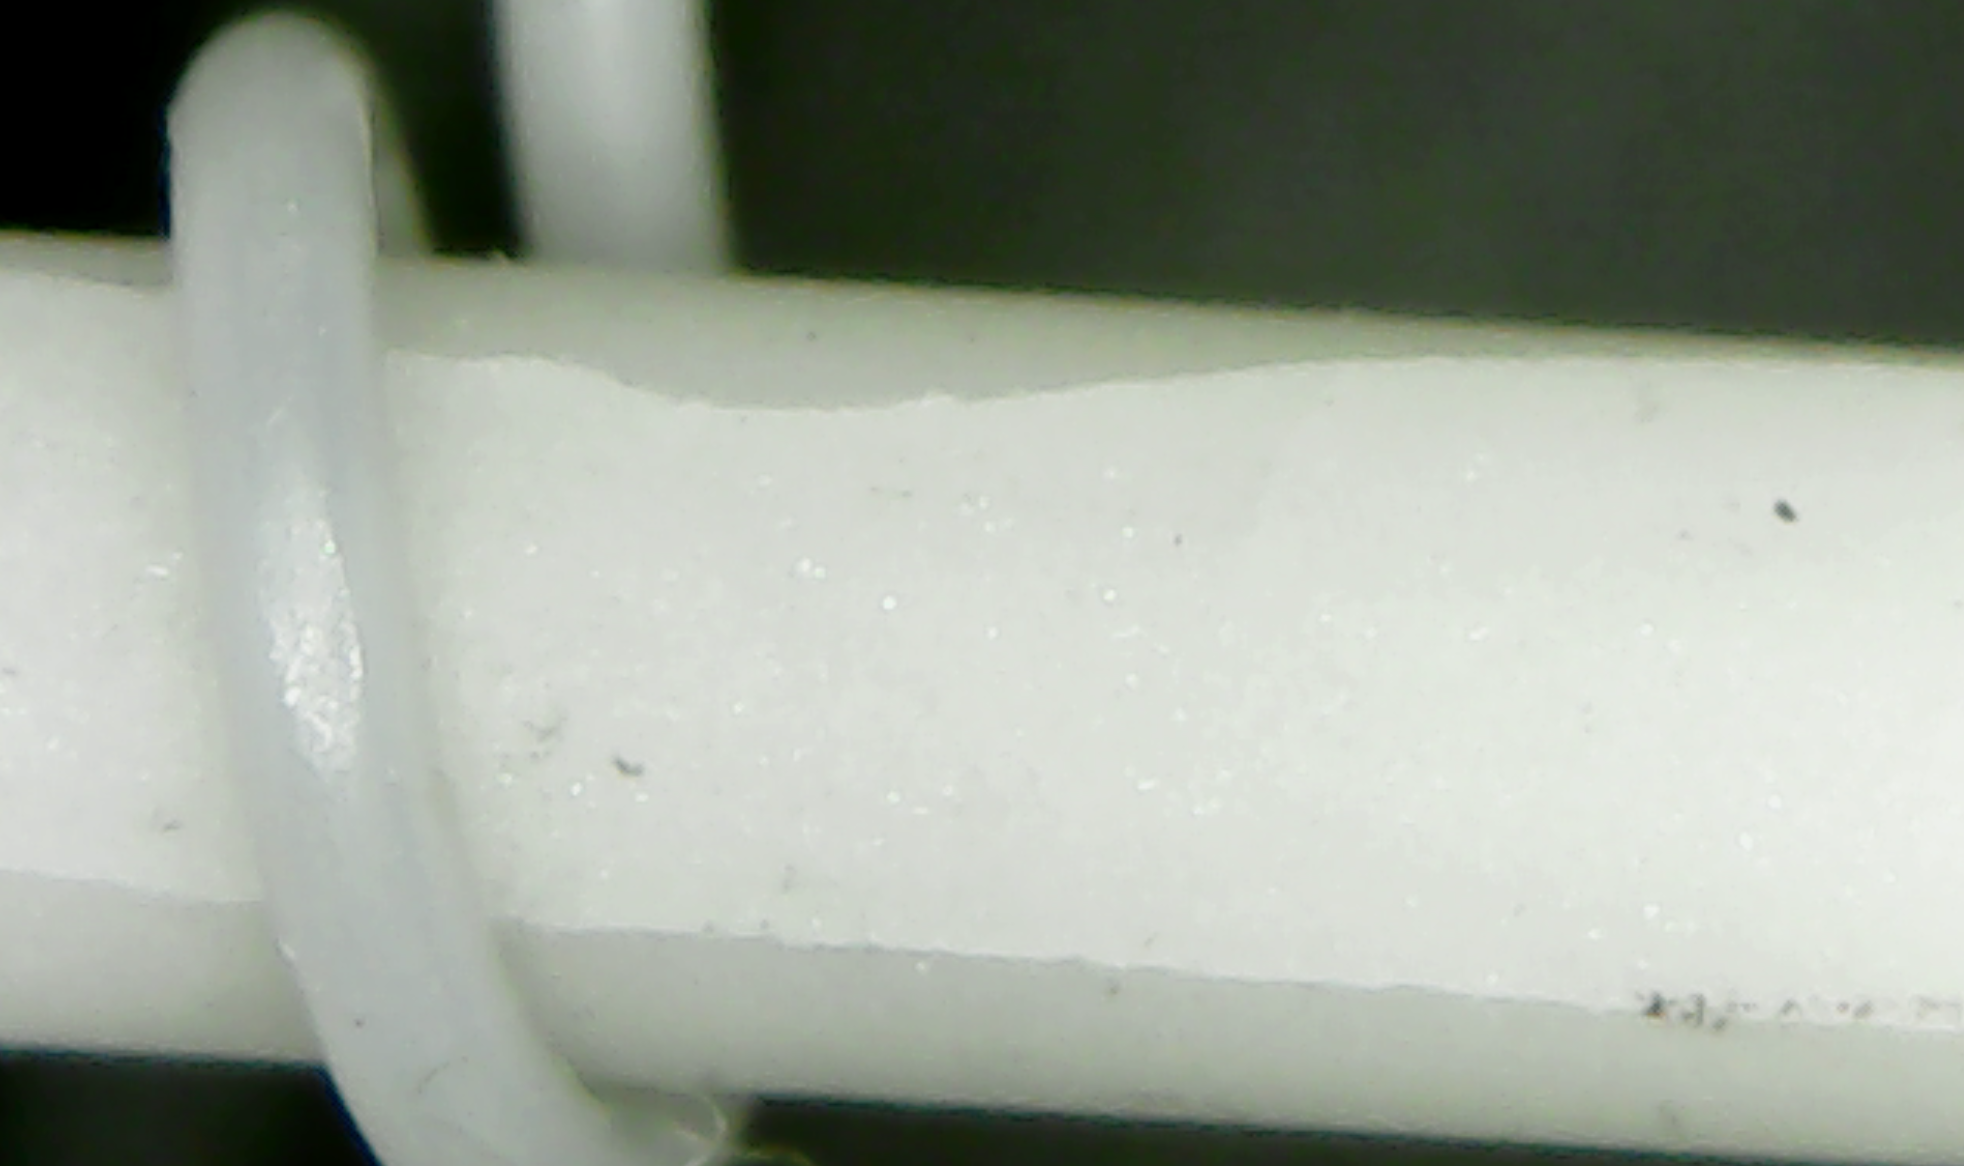
\includegraphics[width=0.6\textwidth]{images/figure_6.png}
\caption{Cracks observed with the microscope in the ceramic of the sensor.
\label{fig:broken_sensor}}
\end{figure}

%%%%%%%%%%%%%%%%%%%%%%
%%%%%%%%%%%%%%%%%%%%%%%

\subsection{Calibration procedure}
\label{sec:calib_procedure}

\noindent The calibration procedure relies on the assumption that all sensors in the capsule are at the same temperature. This limits the number of RTDs in a single run to four, since i) they should be as close as possible to each other and ii) as far as possible from the capsule walls (the sensor closer to the wall could be biased). Two different methods, described schematically in Fig.~\ref{fi:CAL_sequence}, were used to cross-calibrate all 48 sensors in runs of 4 sensors:

\begin{enumerate}
\item {\bf Reference method}: all sensors are calibrated with respect to a reference one, in sets of three sensors (the fourth one would be the reference sensor, which must be present in all runs). In total there are sixteen calibration sets.
\item {\bf Tree method}: Four different sets of sensors can be cross-calibrated by performing a second round of measurements with a single promoted sensor from each of those four sets. Since there are 16 sets in total, a third round of measurement is needed to cross-calibrate the four sets in the second round.
\end{enumerate}

\begin{figure}[htbp]
\centering
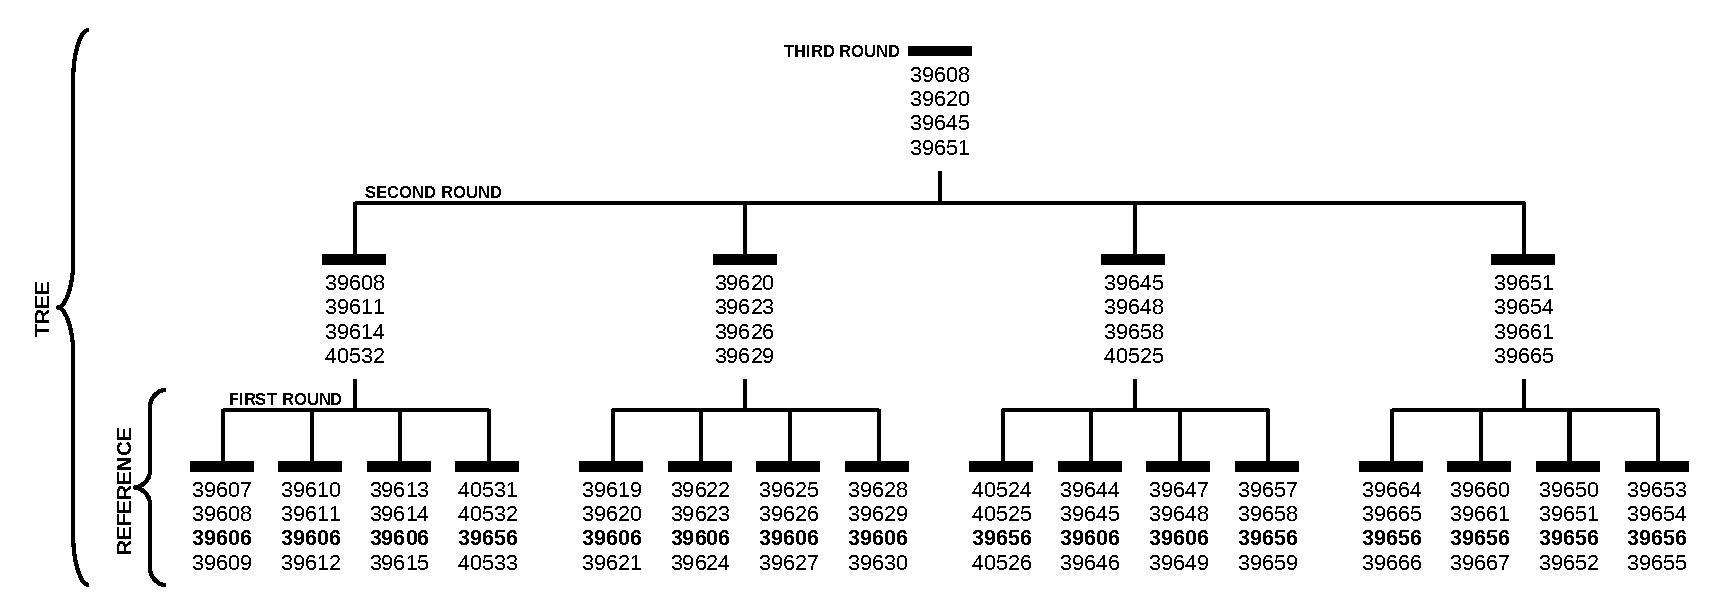
\includegraphics[width=\textwidth]{images/figure_7.pdf}
\caption{Schematic view of calibration sequence. Each number represents a different RTD, and the numbers in bold represent the reference sensors. The first round consists on a direct calibration respect to a reference sensor. The second and third rounds are needed to relate all sensors independently of the reference sensor.
\label{fi:CAL_sequence}}
\end{figure}

The reference method was expected to be more precise since any two sensors were related through a single intermediate sensor (the reference one), while for the tree method the relation between any two sensors required more than one intermediate sensor. For example, the offset between sensors $i$ and $j$ in different sets, related through sensors $k$ and $l$ in the second round, would be $\Delta T_{ij} = \Delta T_{ik} + \Delta T_{kl} + \Delta T_{lj}$. For sensors related through the third round an additional term should be added, further increasing the offset uncertainty.

Offset repeatability is a critical parameter to understand, as the laboratory calibration must remain valid when applied to the actual detector. To study this, four independent calibration runs were performed for each set of four sensors. However, due to concerns about thermal fatigue in the primary reference sensor---subjected to 64 thermal cycles over the four repeatability runs---three secondary reference sensors were employed to regularly monitor its response and ensure reliability over time.

The following procedure is applied for each set of four sensors. First, they are placed inside the aluminium capsule. The central connector closer to the red one is used for the reference sensor. These positions are easily called by numbers from 1 (orange) to 4 (red), as shown in Fig.~\ref{fi:CAL_procedure}-left.

\begin{figure}[htbp]
\centering
\begin{tabular}{ c }
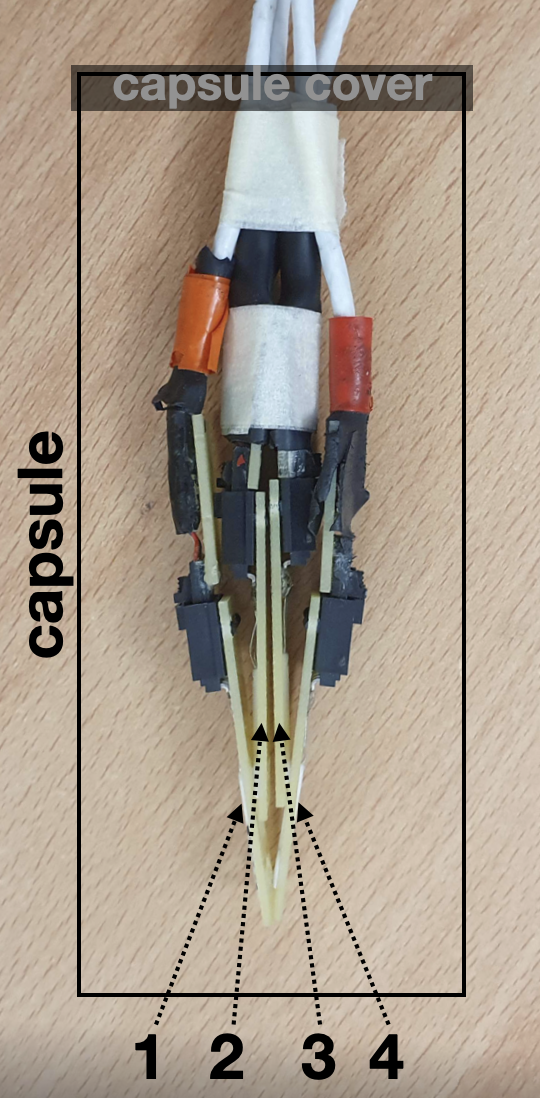
\includegraphics[height=0.34\textheight]{images/figure_8_a.jpg}
\end{tabular}%
\begin{tabular}{ c }
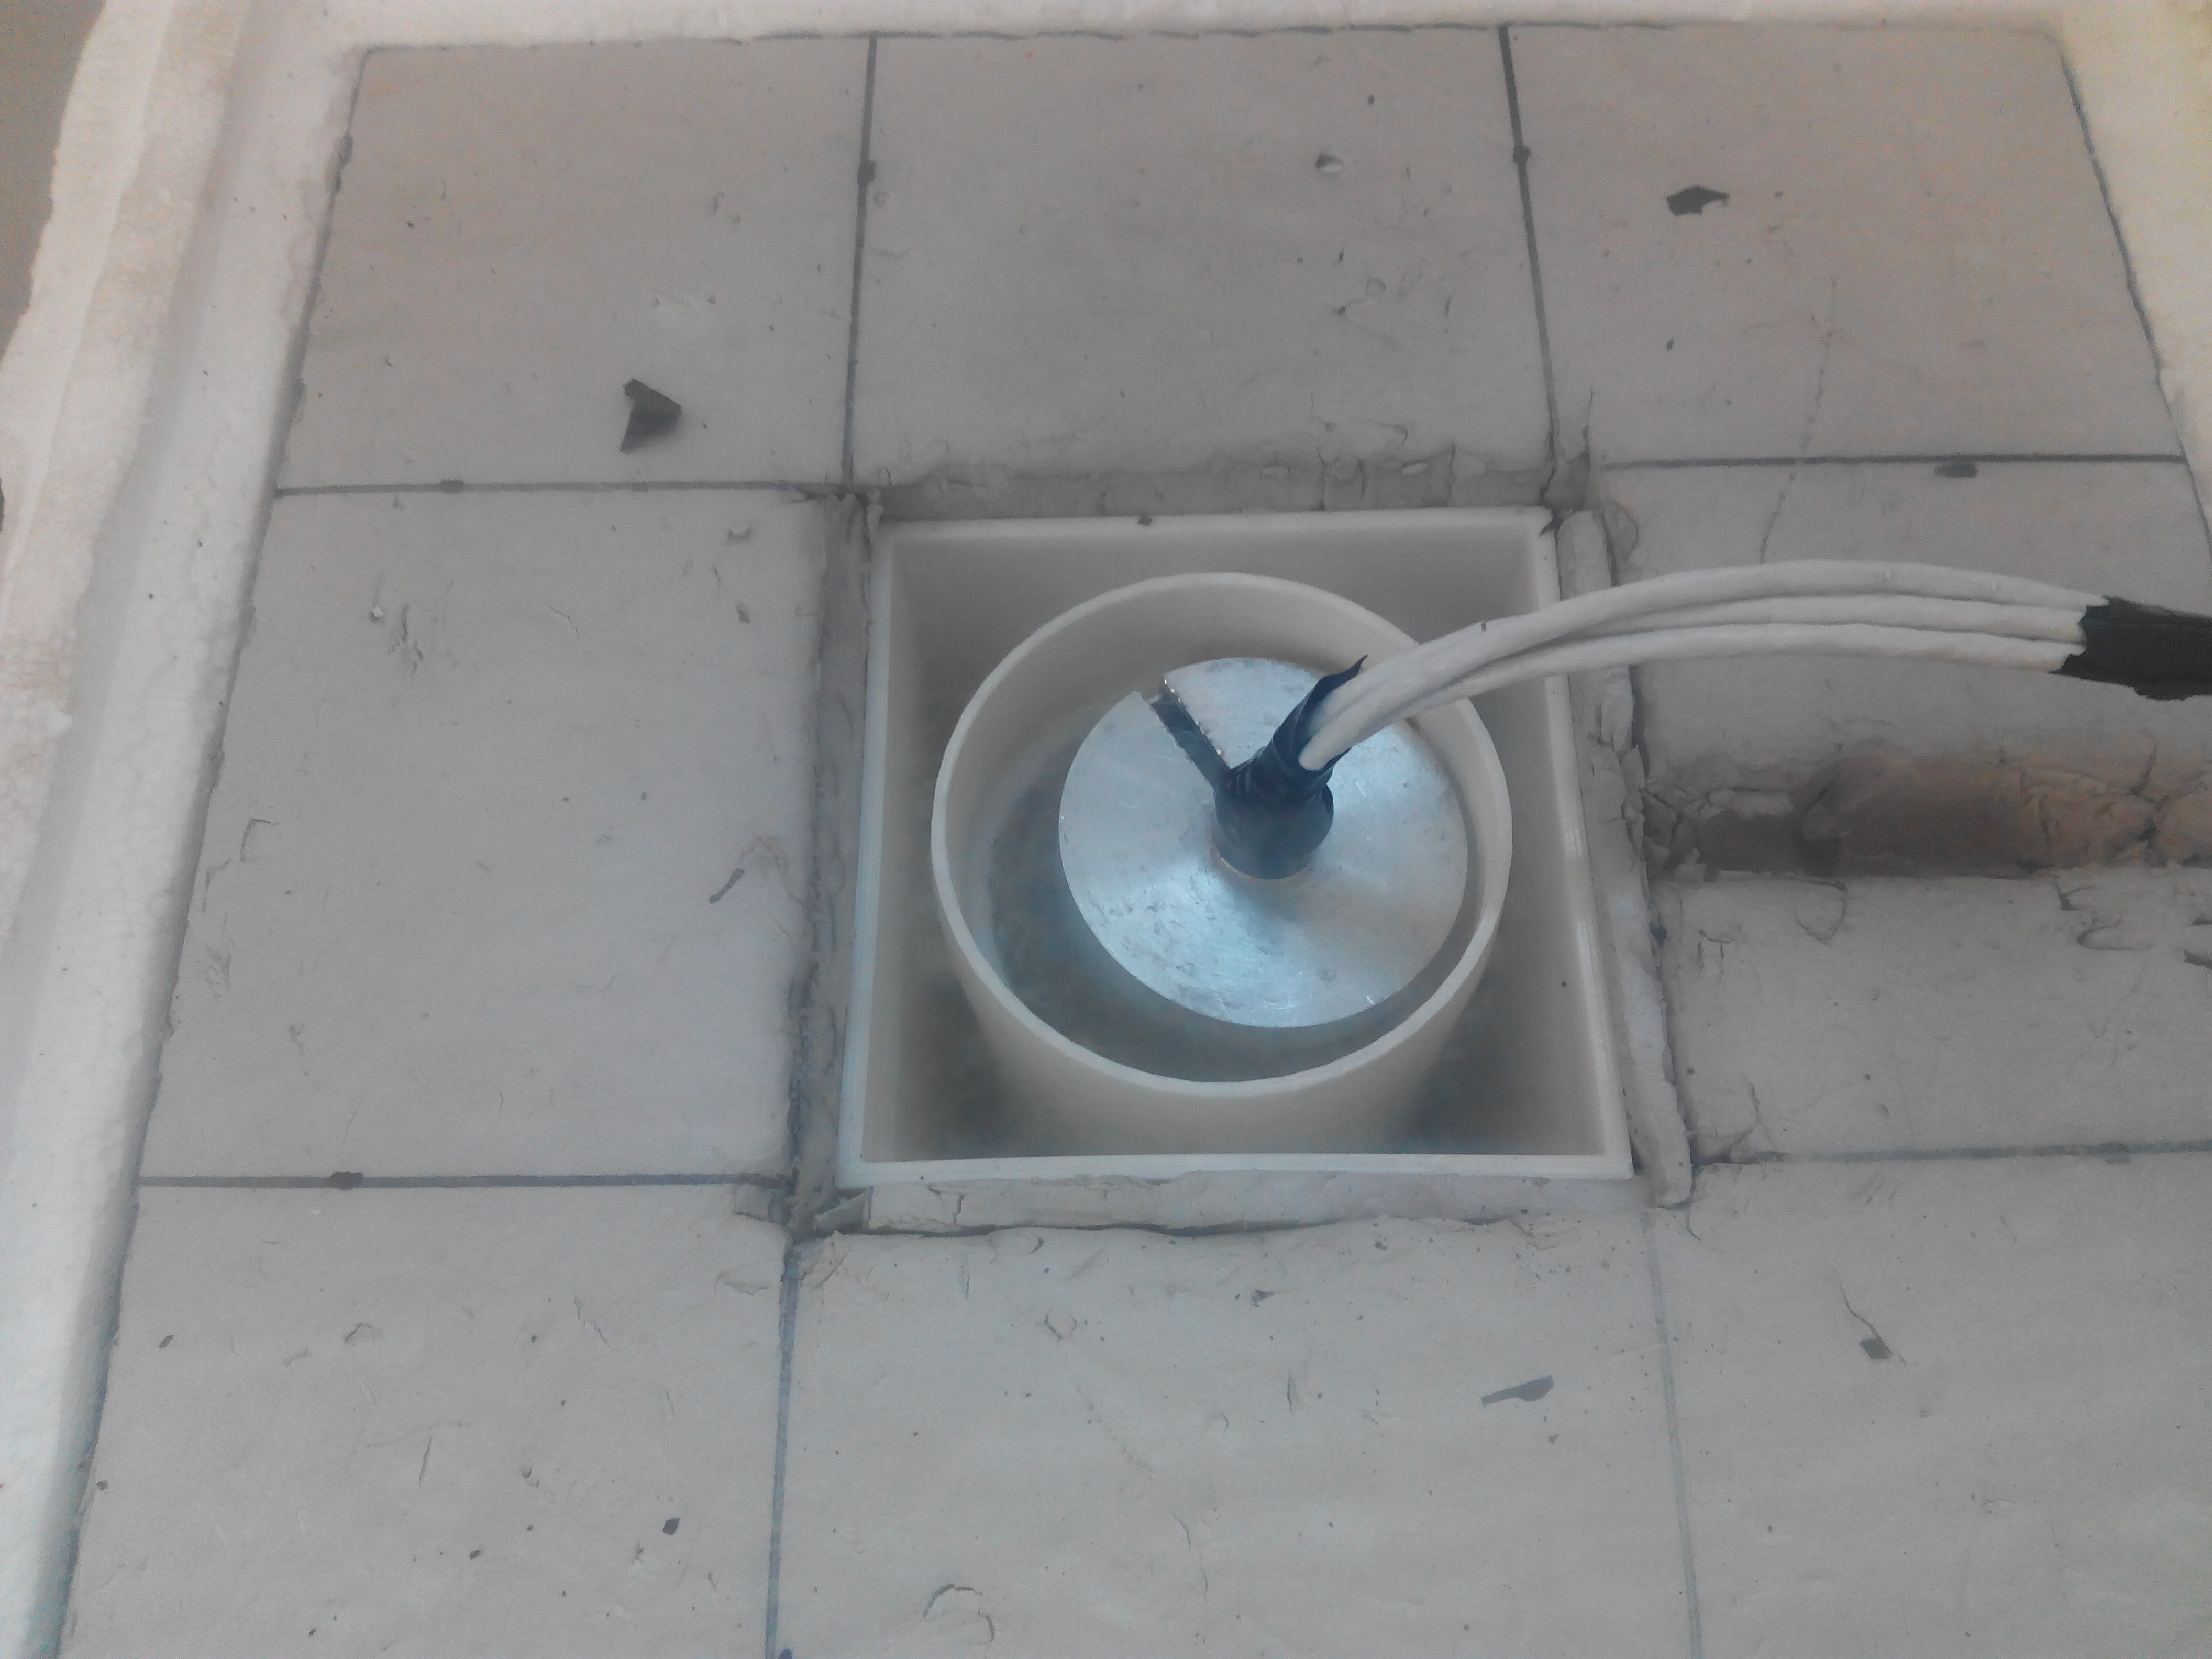
\includegraphics[height=0.1665\textheight]{images/figure_8_b.jpg} \\
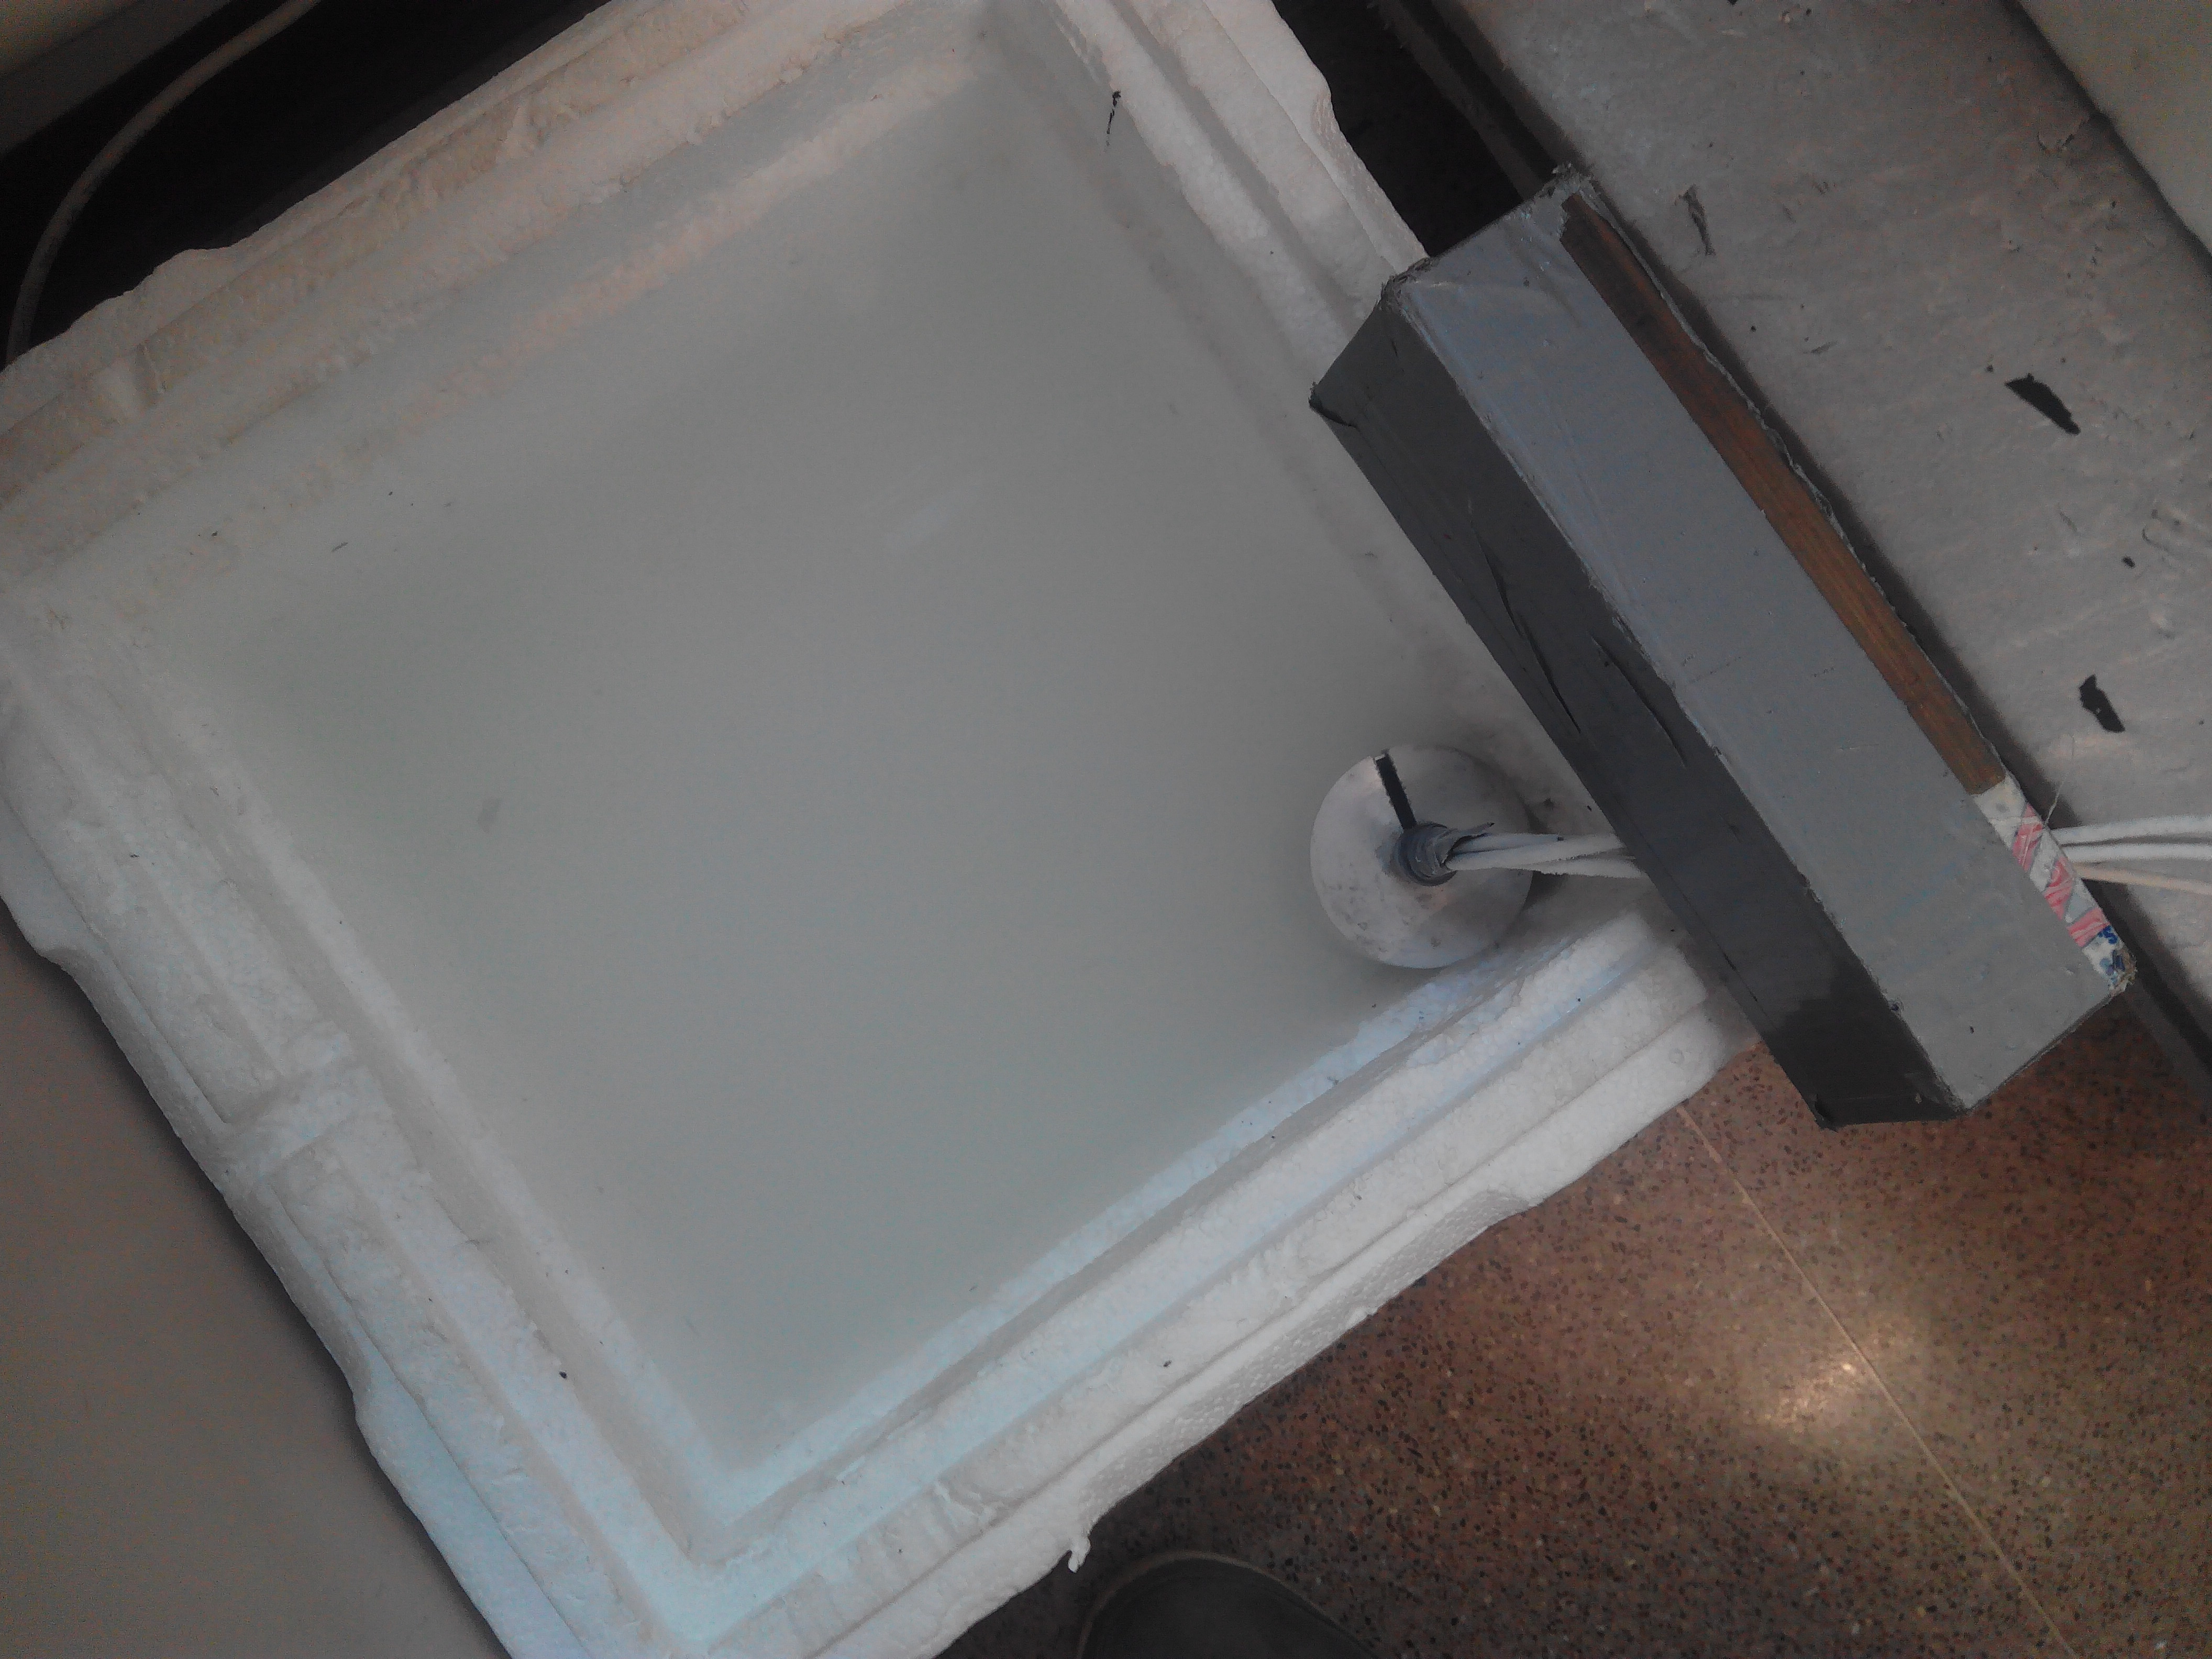
\includegraphics[height=0.1665\textheight]{images/figure_8_c.jpg}
\end{tabular}
\caption{Left: Picture of sensor order inside the flask. Position 1 corresponds to highest serial number and 4 to lowest; position 3 is reserved to reference sensor.
 Top: Flask partially introduced in LAr.
 Bottom: Flask partially introduced in room water to warm up sensors before performing a new measurement.
\label{fi:CAL_procedure}}
\end{figure}

After filling the PLA box with liquid argon, the aluminum capsule is partially immersed (see Fig.~\ref{fi:CAL_procedure}-right-top), allowing the air inside to cool down gradually. This setup prevents the sensors from coming into direct contact with liquid argon, instead inducing a slow cooldown through the surrounding cold gas atmosphere, thereby avoiding thermal shock. When the monitored temperature approaches the one of LAr ($< 95$ K), which takes about 15 minutes, the capsule is completely immersed, being filled with liquid. The PLA box is then completely filled with LAr to account for evaporation during the cool-down phase. Finally, the polystyrene vessel is closed using the polystyrene lid. The calibration run actually begins at that point and lasts for 40 minutes.

When the measurement is finished, the capsule is extracted from the liquid, emptied of LAr and partially immersed into another polystyrene box filled with water at room temperature (see Fig.~\ref{fi:CAL_procedure}-right-bottom). The warm-up process takes about ten minutes. When sensors have reached a temperature around 250 K a new independent calibration run can start.

Fig.~\ref{fi:CAL_pre} shows the typical evolution of the temperature for the four sensors in the capsule during the warm-up and cool-down processes. A sudden fall to 87 K is observed at minute 32, which corresponds to total immersion of the sensors in LAr. Notice also that two of the sensors have lower temperature during the cool-down process; those are sensors 1 and 4, the ones closer to the capsule walls.

For each set of sensors the procedure described above is repeated four times, resulting in four independent measurements of the same offset. These measurements are used to compute a mean offset value and its standard deviation (repeatability from now on).

\begin{figure}[htbp]
\centering
{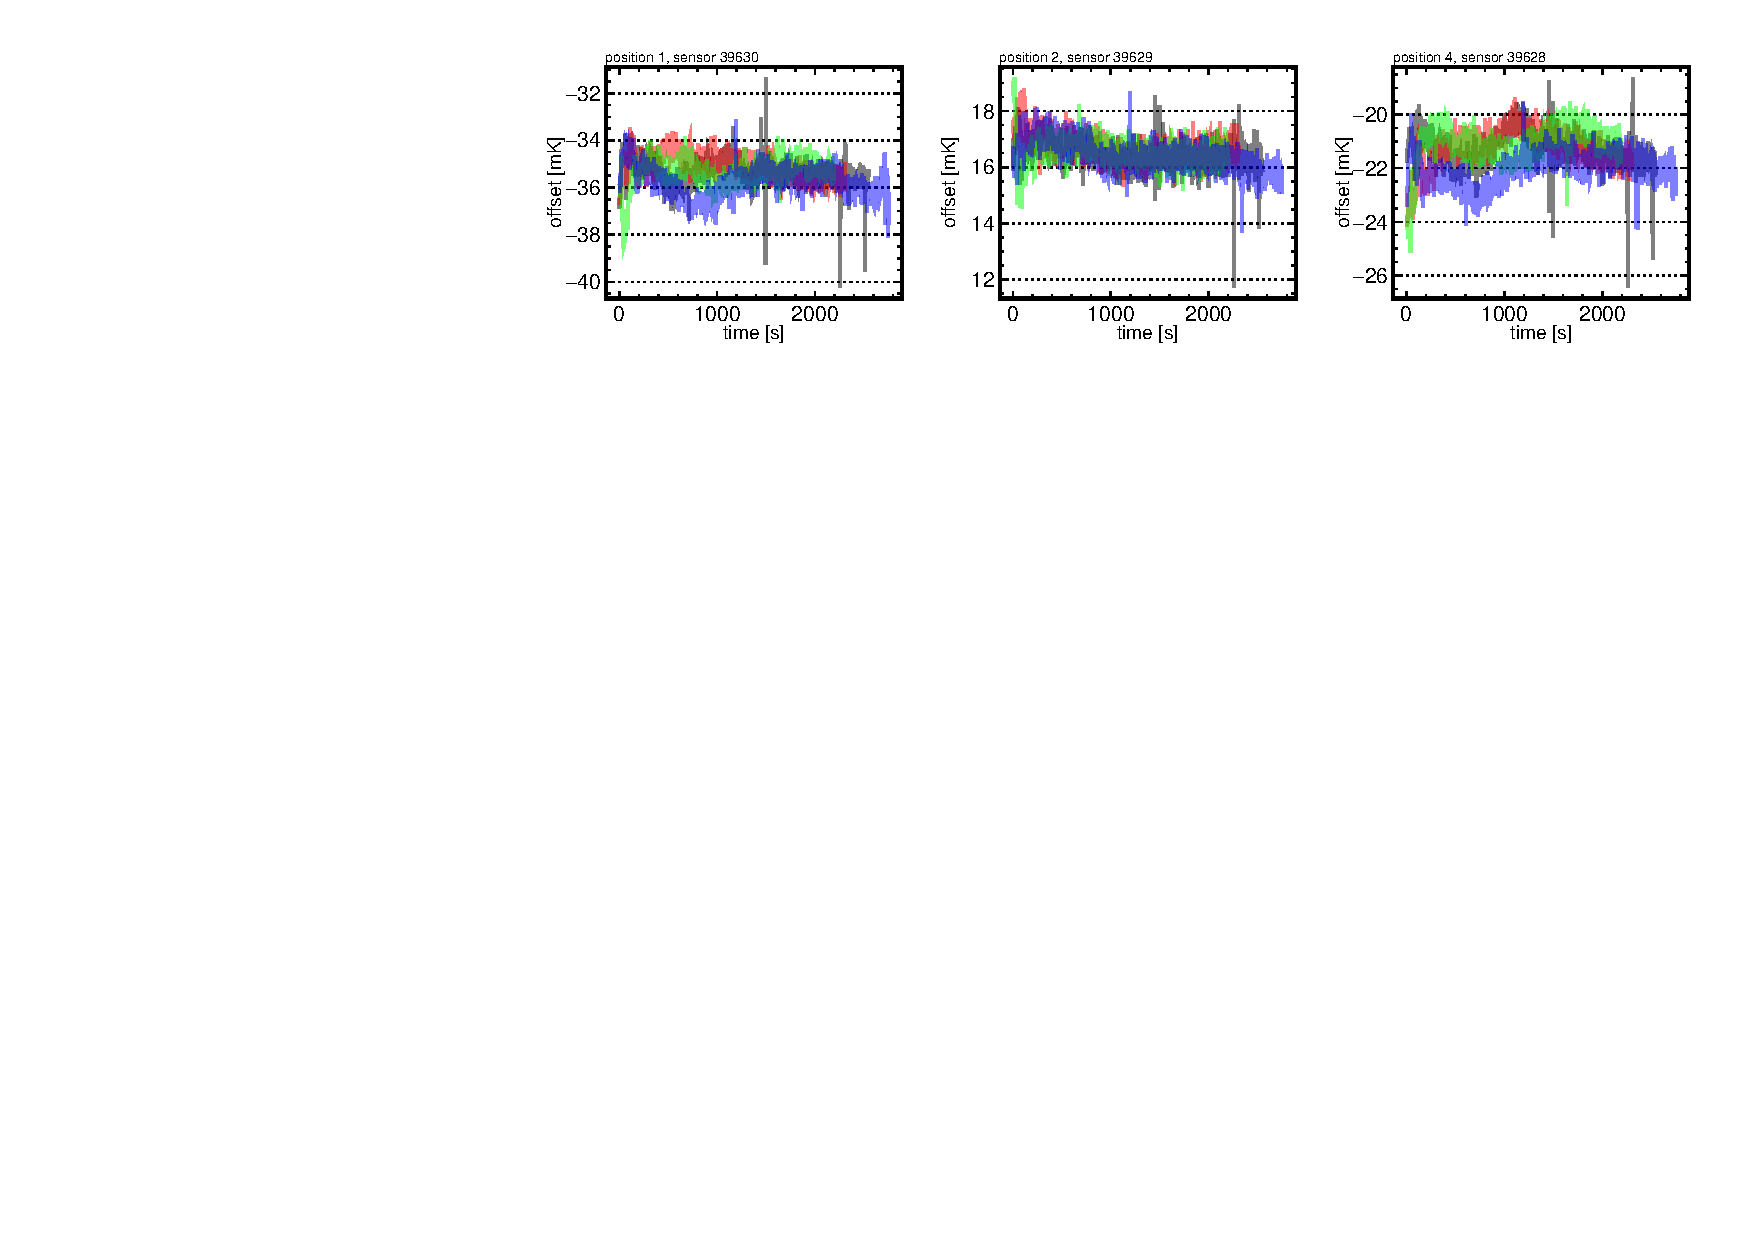
\includegraphics[width=0.6\textwidth]{images/figure_9.pdf}}
\caption{Temperature evolution between two calibration runs, showing the warm-up and cool-down phases of the four temperature sensors inside the capsule. Sensors 1 and 4 are located closest to the capsule walls.}
\label{fi:CAL_pre}
\end{figure}

%%%%%%%%%%%%
%%%%%%%%%%%%

\subsection{Calibration results}
\label{sec:calib_results}
\noindent Here we present the results of the calibration using both calibration methods, a study of the consistency of these results, and a preliminary estimation of the systematic uncertainty of the calibration process.

%---------------------------------------------------
\subsubsection{Results on the first round of measurements}
\noindent Fig.~\ref{fi:CAL_offset_example} shows the offset of three different sensors with respect to the reference sensor as a function of time, and for four independent calibration runs. The offset is more stable for the sensor closer to the reference (position 2), while external sensors (positions 1 and 4) present larger variations, but show similar patterns between them. This effect is attributed to the geometry of the system, with sensors at different heights and not symmetrically positioned with respect to the capsule walls. This was taken into account when developing the second version of the system, presented in Sec.~\ref{sec:new_calib}.

\label{sec:results_first_round}
\begin{figure}[htbp]
\centering
{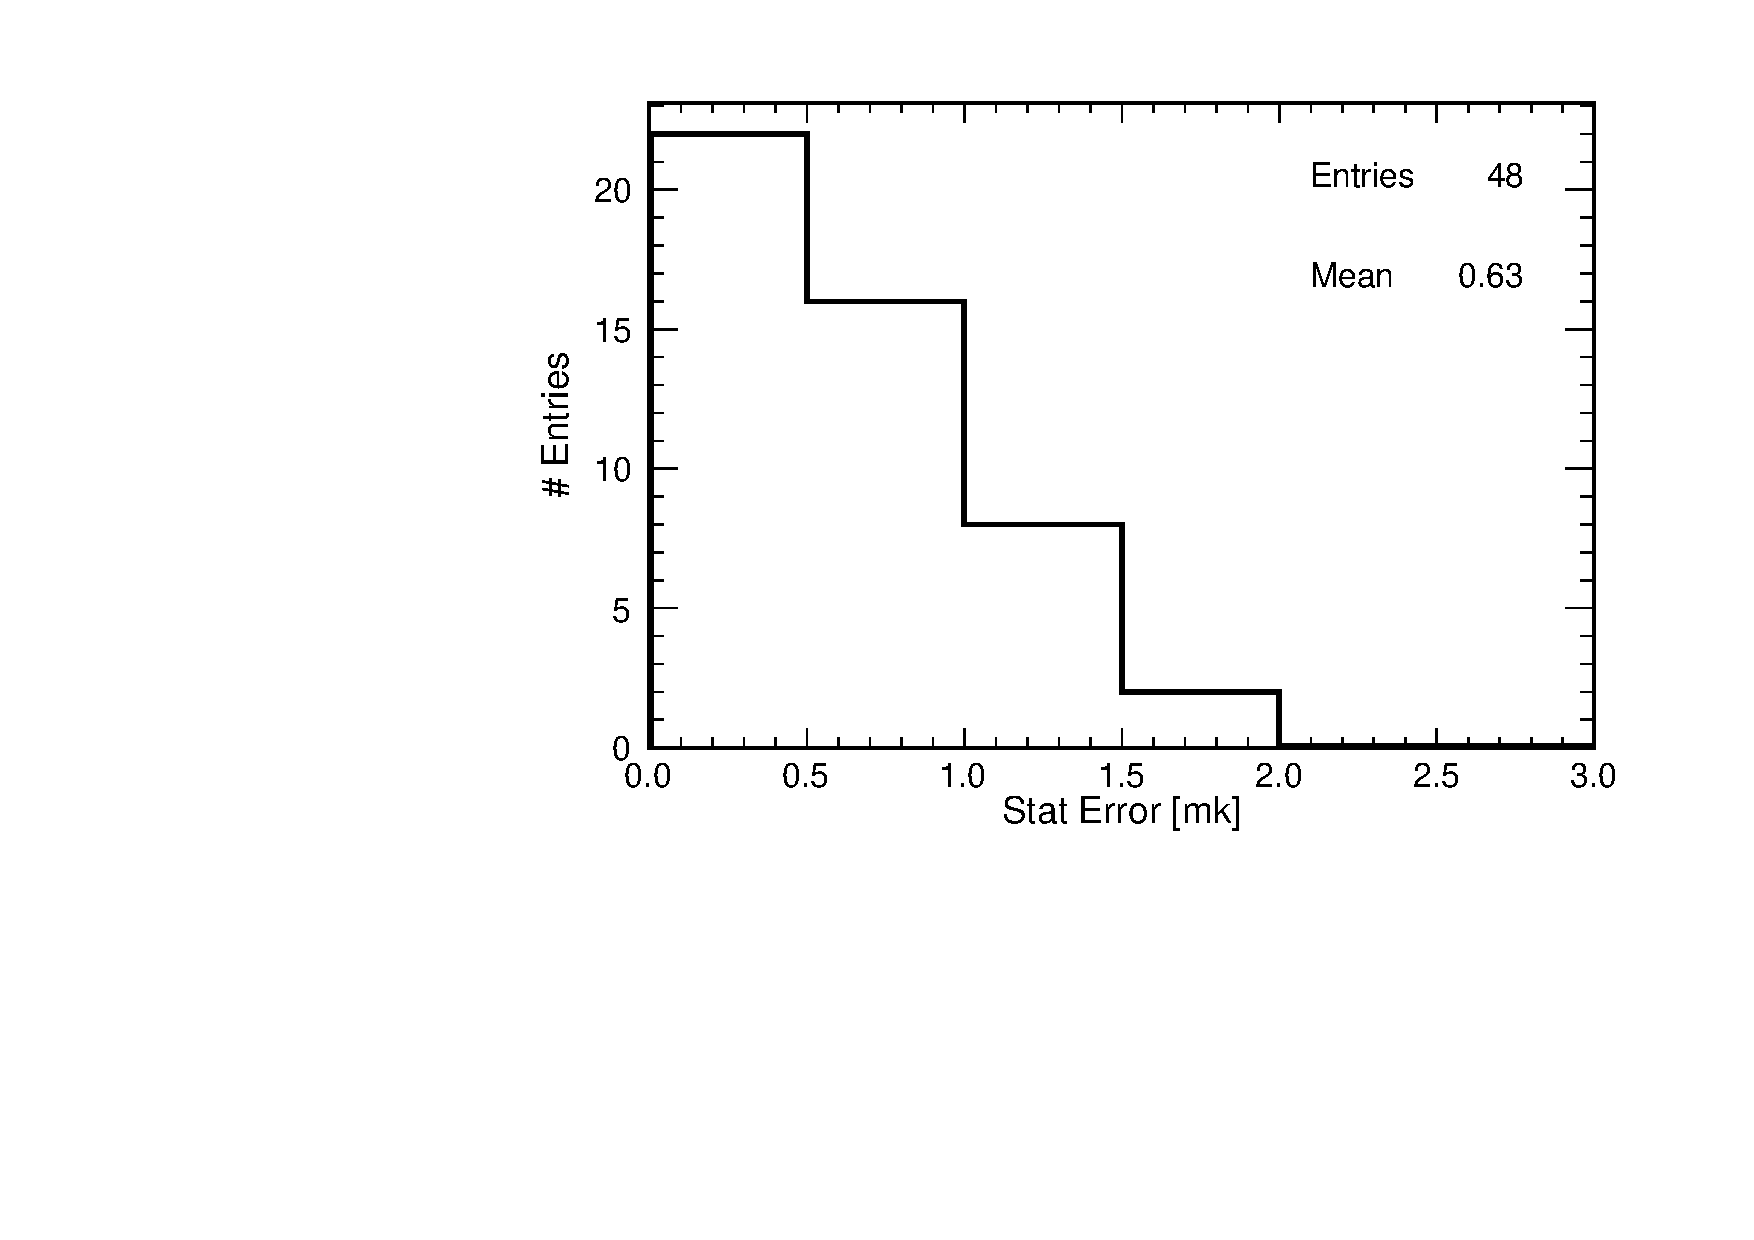
\includegraphics[width=\textwidth]{images/figure_10.pdf}}
\caption{Offset between the reference sensor and each of the three sensors in a set, as a function of time. Each colour represents an independent calibration run.}
\label{fi:CAL_offset_example}
\end{figure}

The mean offset for each sensor and each calibration run is calculated as the average over the time interval between 1000 and 2000 seconds, identified as the most stable region for the majority of the runs. The standard deviation of the four means is taken as the uncertainty, hereafter referred to as repeatability. As shown in Fig.~\ref{fi:CAL_rms_1r}, the uncertainties are generally below 1~mK, demonstrating the high level of repeatability achieved in the calibration process.

\begin{figure}[htbp]
\centering
{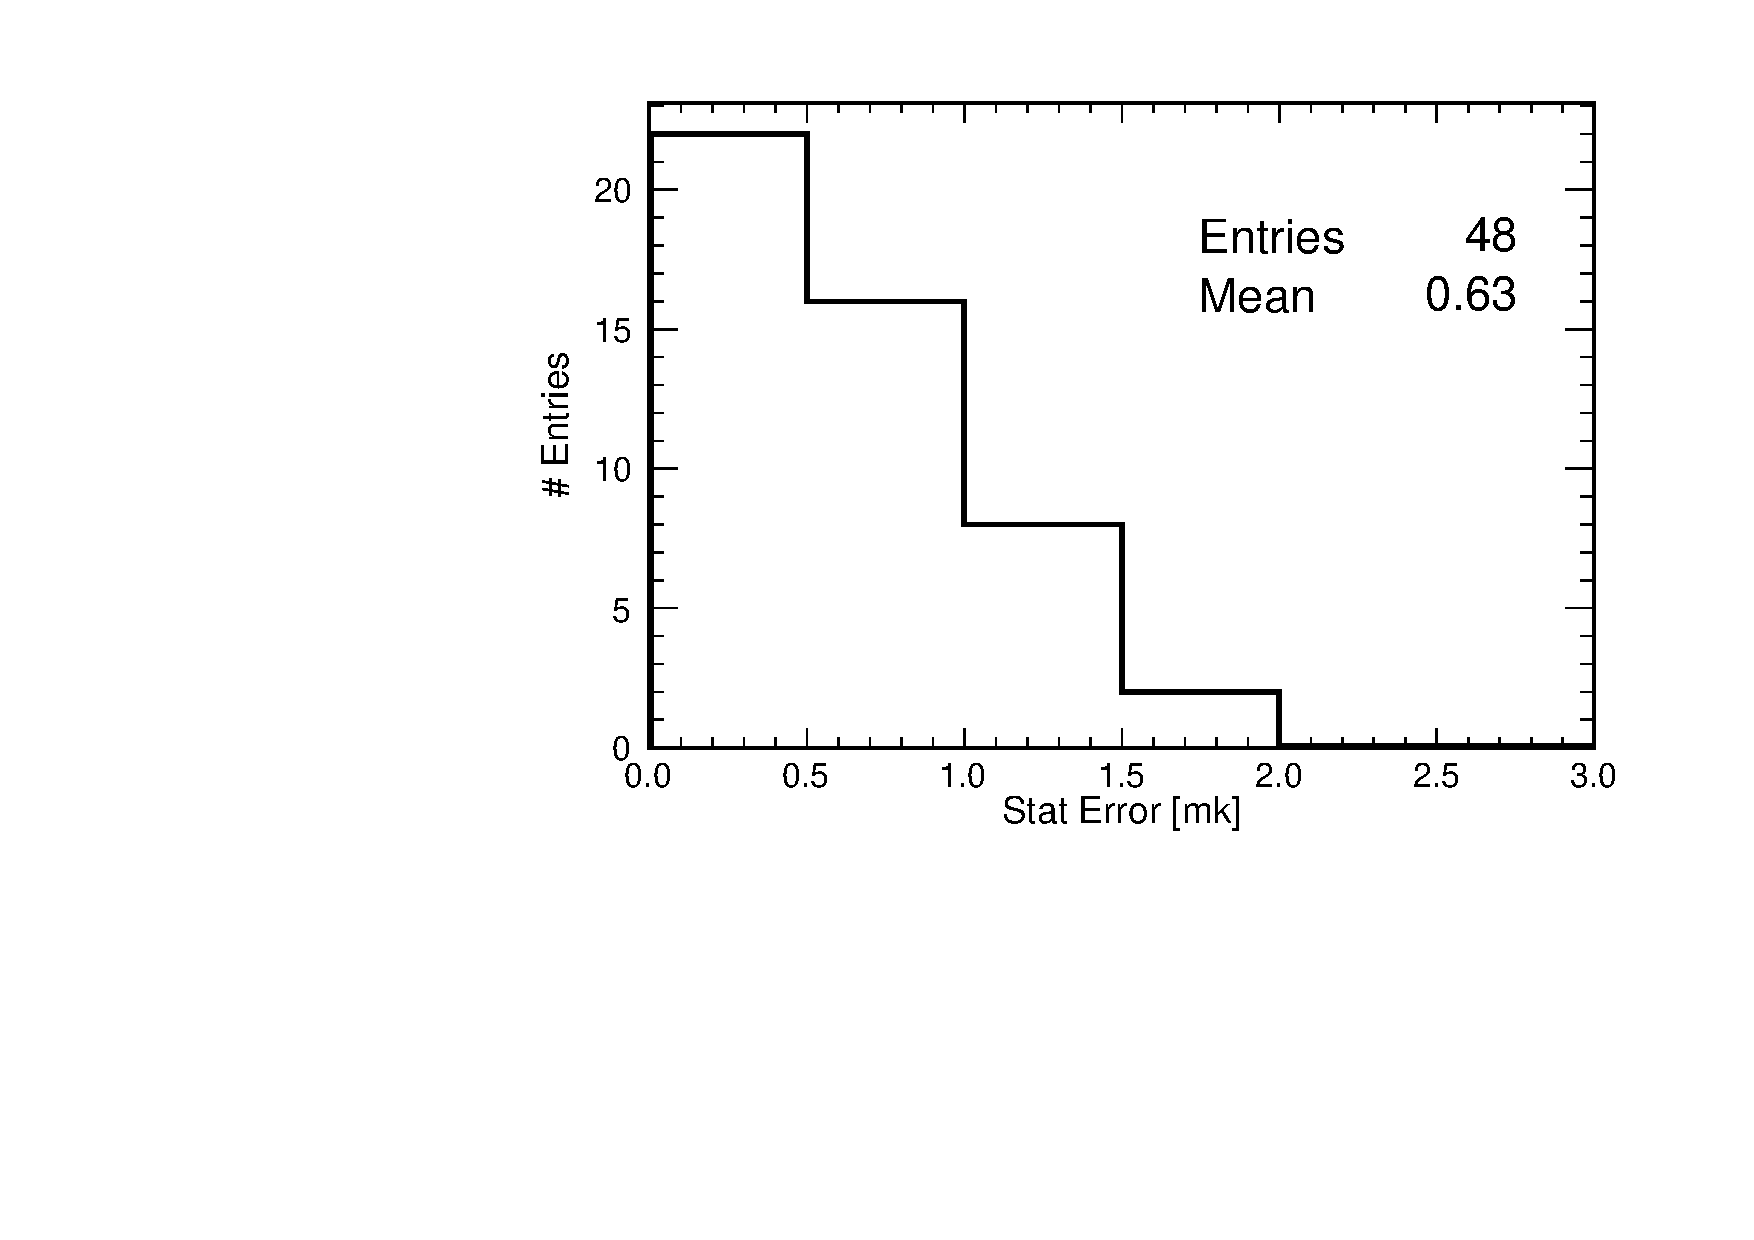
\includegraphics[width=0.6\textwidth]{images/figure_11.pdf}}
\caption{Distribution of the repeatability for calibration runs in the first round.}
\label{fi:CAL_rms_1r}
\end{figure}

%---------------------------------------------------
%\subsubsection{Evolution on the response of the reference sensors}
\subsubsection{Time walk correction for reference sensors}
\label{sec:reference_corrections}
\noindent Time evolution of the response of sensor 39606 was studied by periodically (every $\sim$20 immersions)  computing its offset with respect to three secondary reference sensors, 39603, 39604 and 39605. For each of those additional calibrations, two runs were taken instead of four in order to minimize thermal fatigue of the reference sensor. As shown in Fig.~\ref{fig:offset_ref}-left, the offset, computed as the mean of those two runs, varies linearly at a rate of 0.07 mK/immersion, which suddenly increases to 0.22 mK/immersion after 60 runs. This change in the slope may be related with to the frequency of immersions, which increased from 3/day to 5/day. Sensor 39606 was initially used for other purposes, and the calibration of the 48 sensors conforming the static TGM started approximately at immersion 40. Given this change in its response, sensor 39606 was substituted by 39656 as primary reference for the last quarter of the TGM calibration in order to avoid further fatigue and potential untraceable behaviour. The evolution of the new reference sensor is shown in Fig.~\ref{fig:offset_ref}-right. It is worth noting that the same slopes are valid for the three secondary reference sensors in both cases, supporting the idea that the change observed in the offsets can be exclusively attributed to thermal fatigue of the reference sensor.

\begin{figure}[htbp]
\centering
{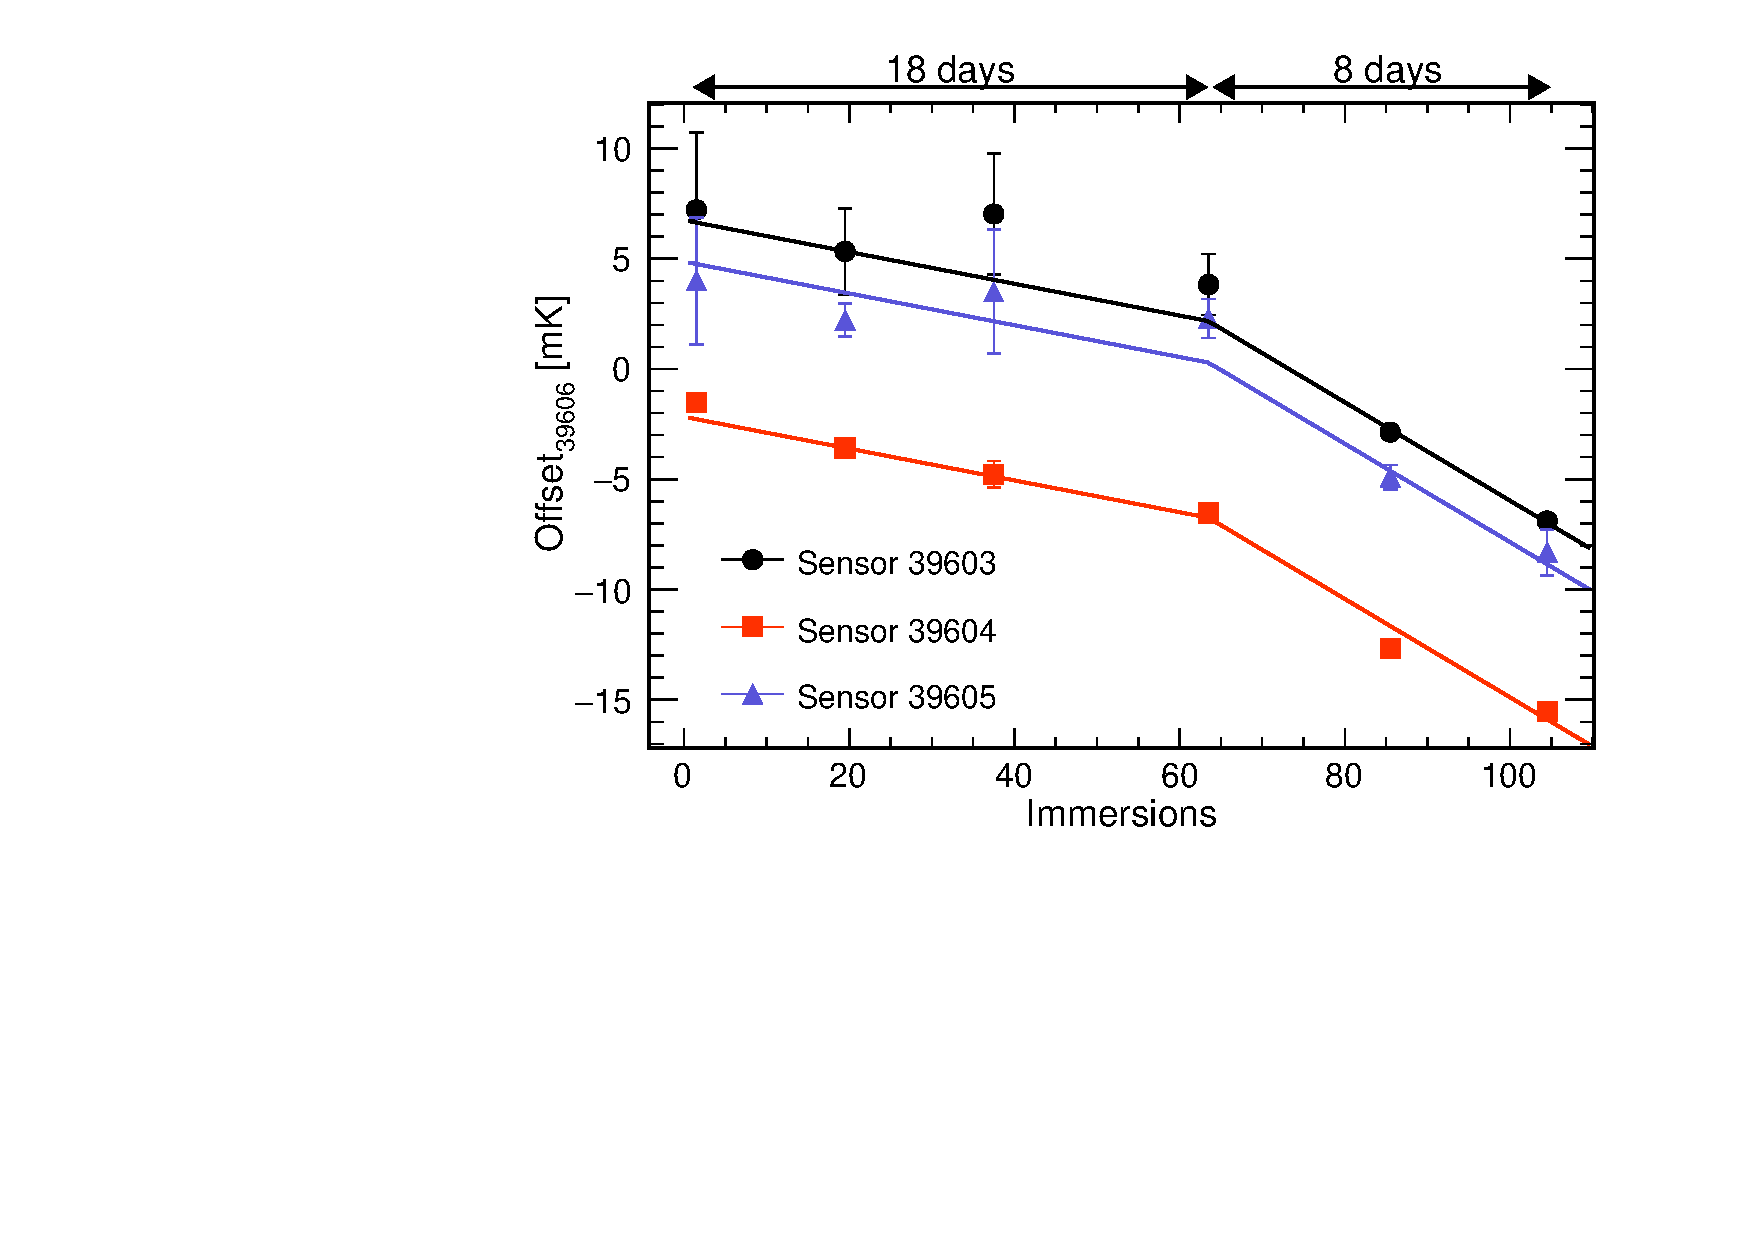
\includegraphics[width=0.48\textwidth]{images/figure_12_a.pdf}}
{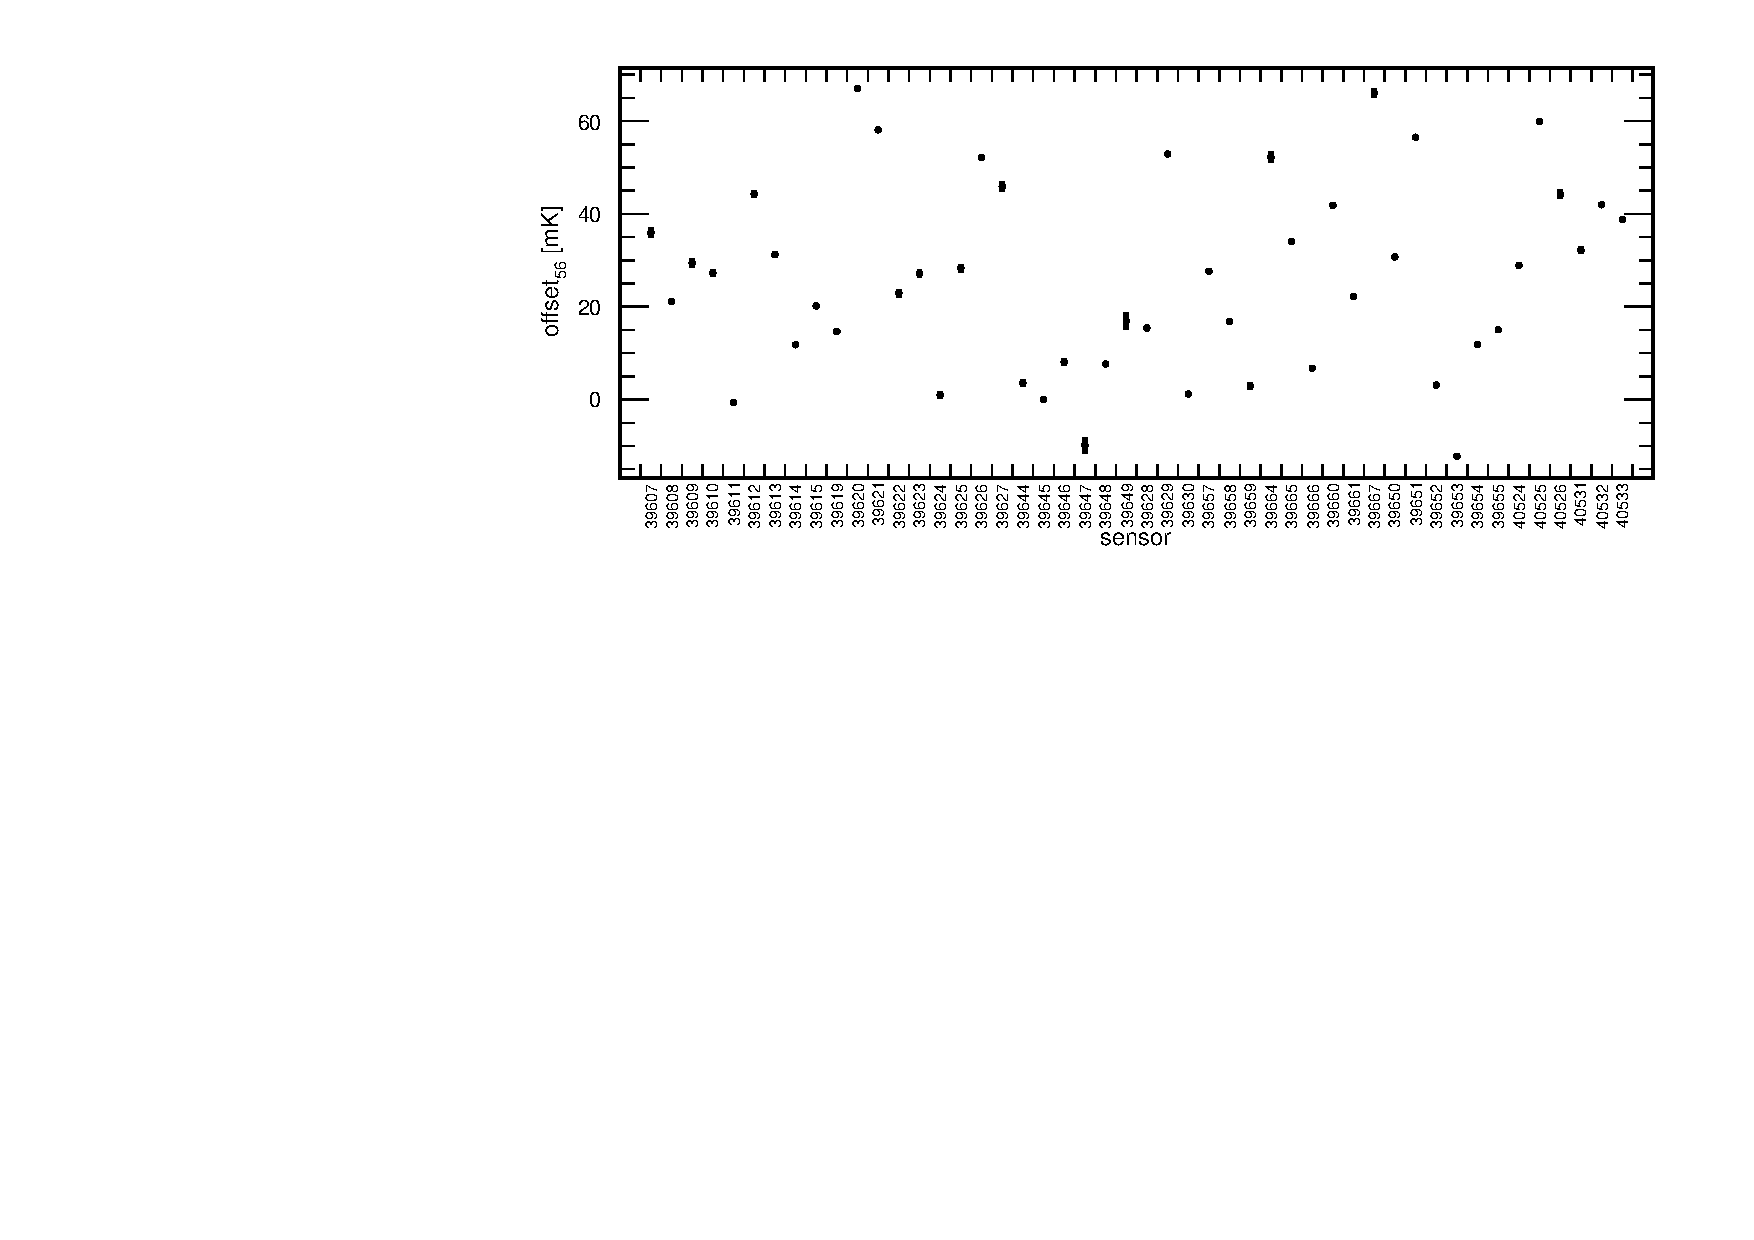
\includegraphics[width=0.48\textwidth]{images/figure_12_b.pdf}}
\caption{Offset between the reference sensors (39606 on the left panel and 39656 on the right panel) and the three secondary references as a function of the number of immersions. Offsets for sensor 39604 have smaller errors because of its position inside the capsule. Solid lines correspond to the parametrization in Eq.~\ref{eq:ref1_param}.}
\label{fig:offset_ref}
\end{figure}

The zero intercept in both panels of Fig.~\ref{fig:offset_ref} corresponds to the unbiased offset (or the offset at $N_{inmersions}=0$) of each of the secondary reference sensors with respect to the primary reference. In order to compute the unbiased offset for a sensor $s$, a time walk correction after $N$ immersions is parameterised as:

\begin{equation}
\Delta T_{s,06}(N=0)=
    \begin{cases}
        \Delta T_{s,06}(N)+(0.072\pm0.003)*N                             & N<63.5\\
        \Delta T_{s,06}(N)+(0.072\pm0.003)*63.5+\\+(0.223\pm0.007)*(N-63.5) & N>63.5 \,,
    \end{cases}
    \label{eq:ref1_param}
\end{equation}

\begin{equation}
\Delta T_{s,56}(N=0)=\Delta T_{s,56}(N)+(0.168\pm0.007)*N  \, .
\label{eq:ref2_param}
\end{equation}

All sensors can be related to the same primary reference sensor, 39606, adding  the unbiased offset between sensors 39606 and 39656,  $\Delta T_{56,06}(N=0)$, to sensors calibrated with respect to 39656. By averaging over the three secondary reference sensors, the value obtained is $\Delta T_{56,06}(N=0)=-9.19\pm0.13$ mk.

%---------------------------------------------------
\subsubsection{Results on the reference method}
\label{sec:results_reference}
\noindent Fig.~\ref{fig:offsets_tree_1} shows the offset of all sensors with respect to the 39606 reference. As it can be noticed, the dispersion of the offsets is compatible with 0.1 K, the value quoted by the vendor. Fig.~\ref{fig:offsets_tree_2}-left shows the distribution of the repeatability of the computed calibration constants after applying the different corrections, showing an average value below 1 mK.

%---------------------------------------------------
\subsubsection{Results on the tree method}
\noindent The offsets are computed in this case with respect to an arbitrary reference among all sensors being calibrated. Selecting as reference a sensor present in the third round (see Fig.~\ref{fi:CAL_sequence}) minimizes the number of operations required to compute the offsets, thereby reducing the associated uncertainty. Sensor 39645 was chosen as reference. Fig.~\ref{fig:offsets_tree_2}-right shows the distribution of the repeatability of the computed calibration constants, the mean of which is slightly below the one obtained for the reference method. Thus, it is confirmed that despite the higher number of intermediate sensors to relate any two sensors, the additional uncertainty introduced by the time walk correction makes the tree method superior to the reference method. Moreover, the reference method introduces a ---not yet known--- systematic error associated to the time wall correction model.

\begin{figure}[htbp]
\centering
{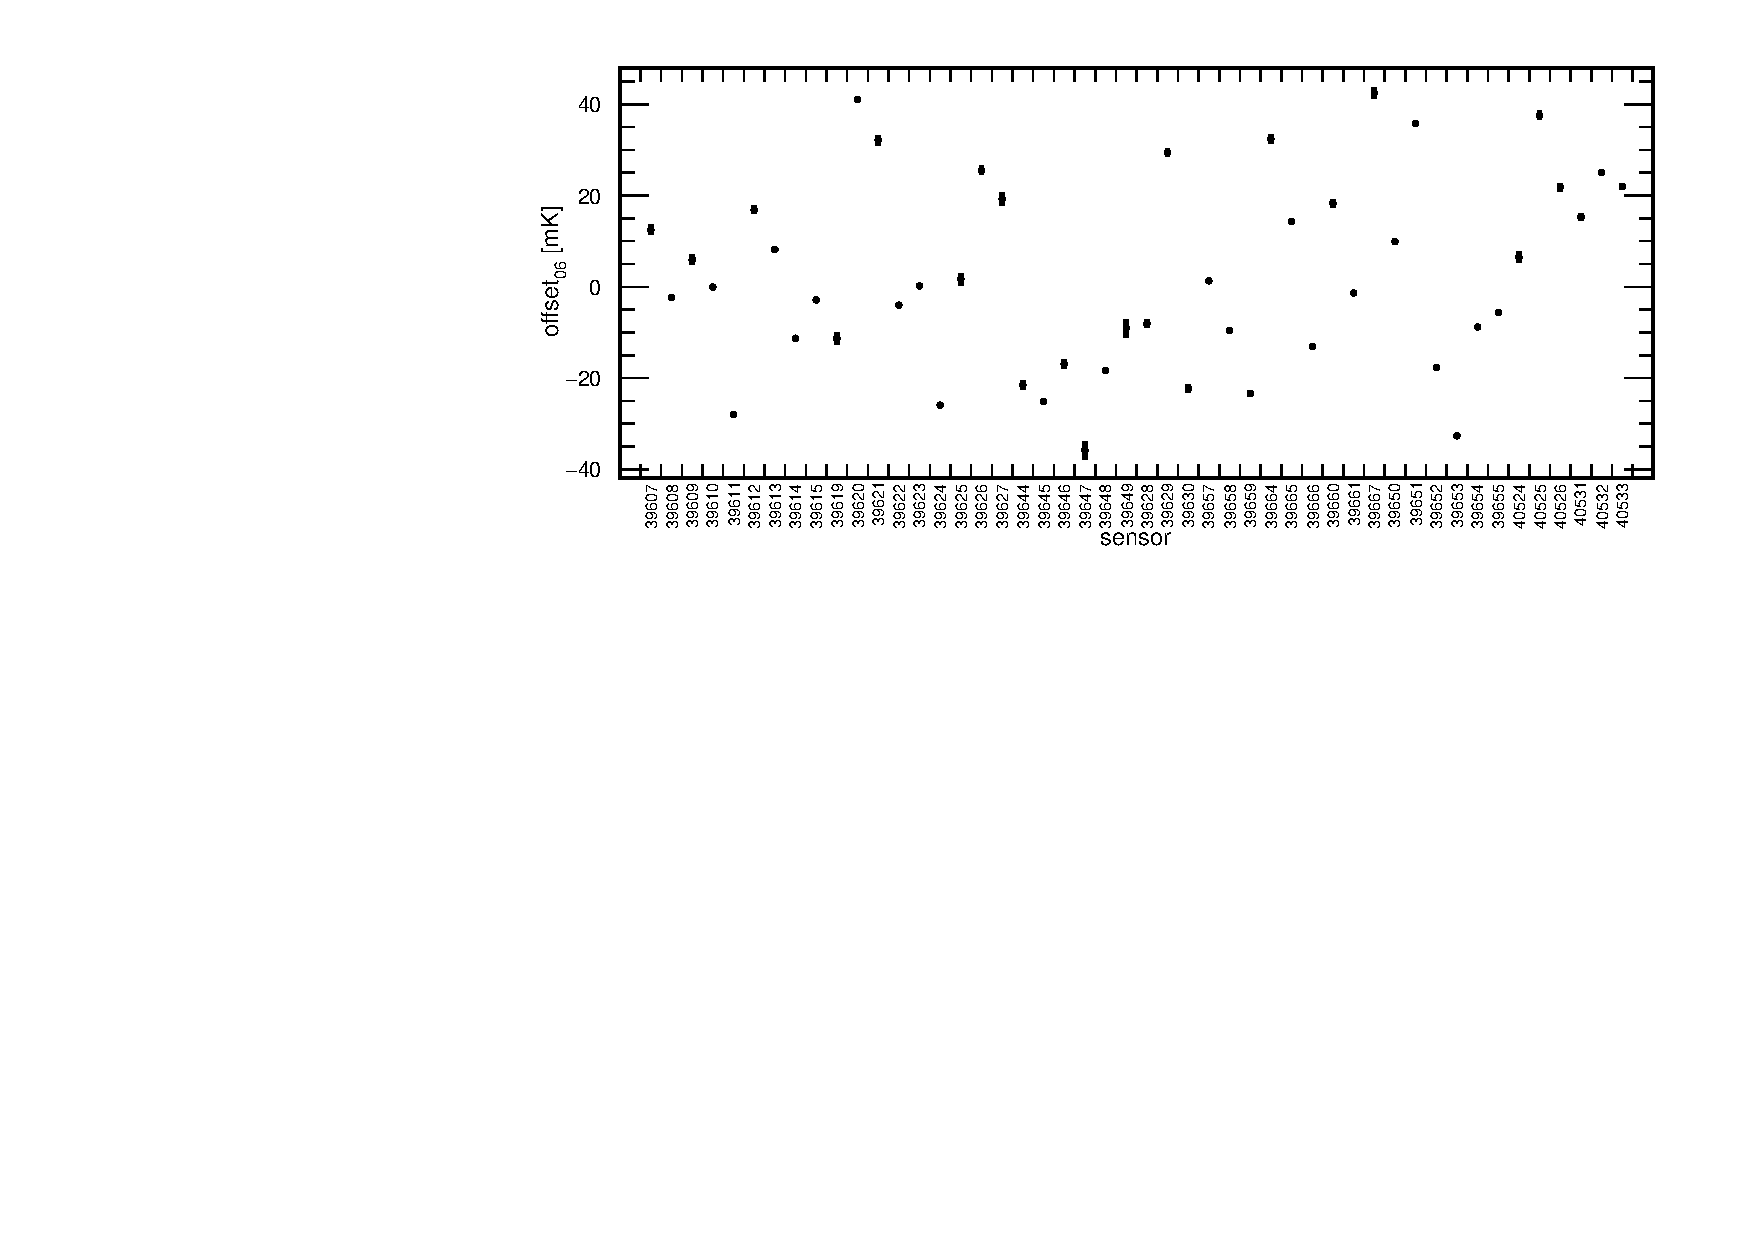
\includegraphics[width=0.9\textwidth]{images/figure_13.pdf}}
\caption{Offset of each sensor with respect to reference sensor 39606 using the reference method.}
\label{fig:offsets_tree_1}
\end{figure}

\begin{figure}[htbp]
\centering
{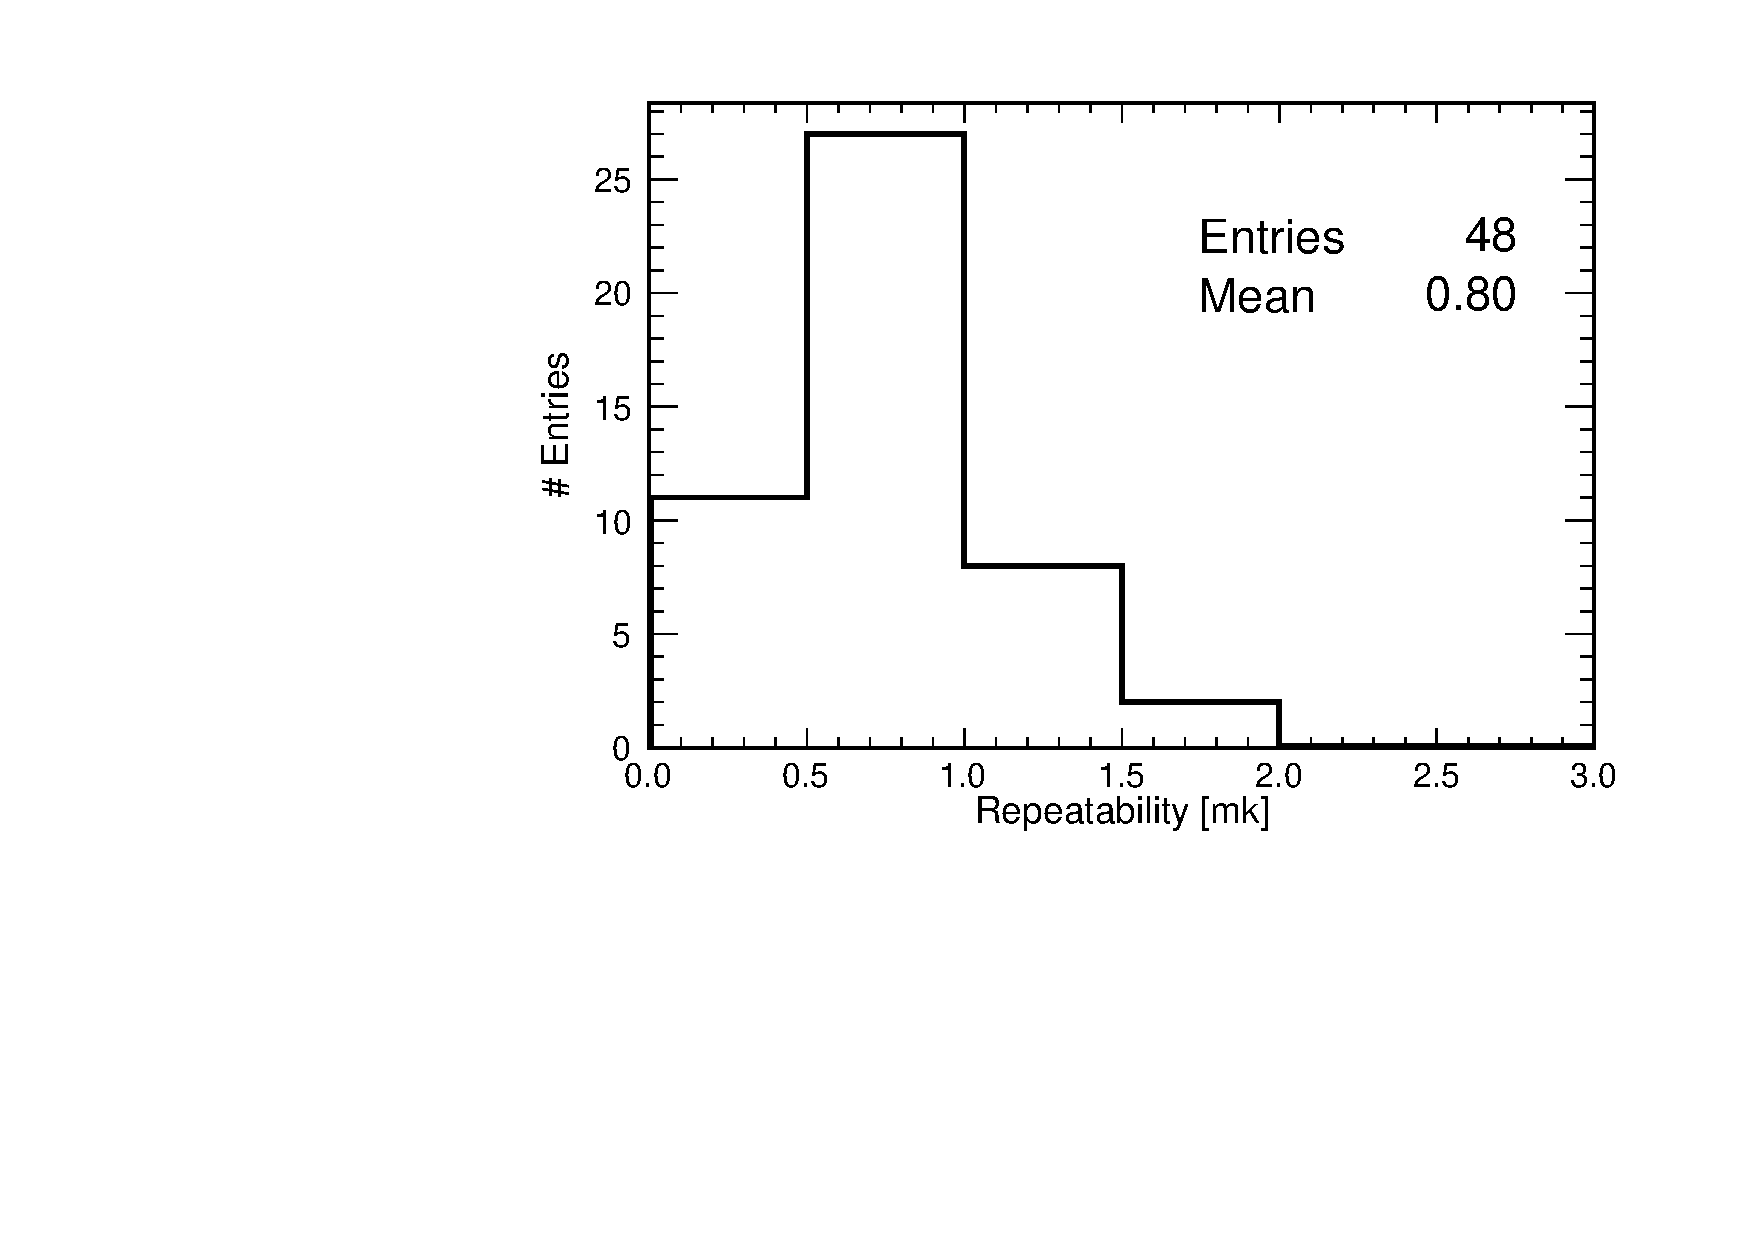
\includegraphics[width=0.45\textwidth]{images/figure_14_a.pdf}}
{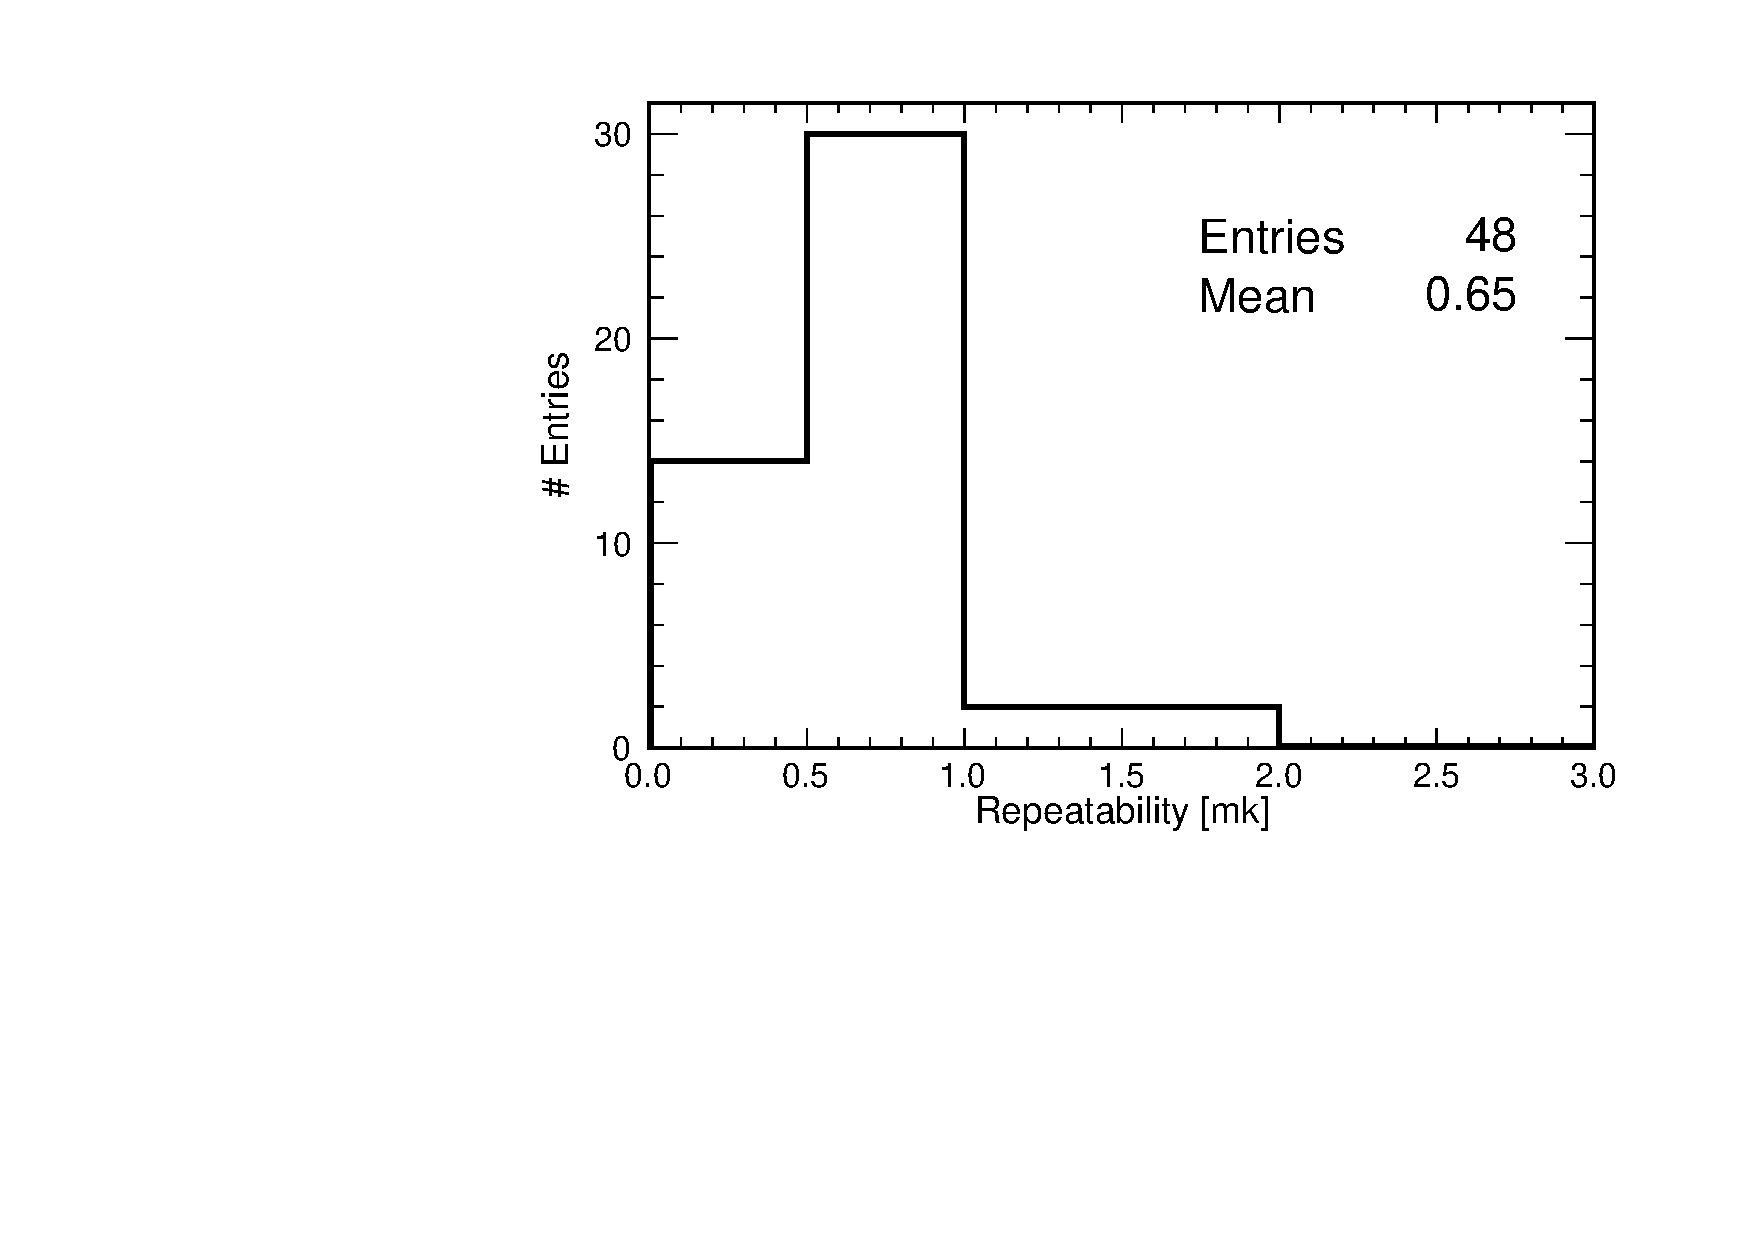
\includegraphics[width=0.45\textwidth]{images/figure_14_b.pdf}}
\caption{Left: repeatability distribution for the reference method. Right: repeatability distribution for tree method.}
\label{fig:offsets_tree_2}
\end{figure}

%---------------------------------------------------
\subsubsection{Consistency cross-check and error estimation}
\label{sec:crossCheck}
\noindent The uncertainties presented are, on average, smaller than 1~mK and correspond to the standard deviation of the four independent measurements of each calibration constant, combined with the error propagation from the required corrections: time-walk correction for the reference method, addition of calibration constants for the tree method, and the uncorrected electronic residual offset common to both calibration methods. These corrections likely include unknown systematic effects impacting the final calibration constants, \textcolor{red}{which need to be added to the systematic uncertainty associated to the assumption of homogeneous temperature inside the capsule}. To estimate the overall precision of the calibration, the following cross-check was performed. The calibration strategy yields two independent values for each sensor’s calibration constant—one obtained from the reference method and the other from the tree method. For the sixteen sensors used in the second round of the calibration tree, these two values are linearly independent because they are derived from different sets: the reference method relies solely on first-round runs, while the tree method uses only second and third-round runs for those sensors. Therefore, these sixteen sensors provide an effective basis for estimating the calibration procedure’s precision by comparing the results obtained from the two methods.

By construction, the result of subtracting the calibration constants obtained in the two methods should be compatible with the offset between sensors 39645 and 39606, $\Delta T_{45,06} = \Delta T_{s,06}-\Delta T_{s,45} = T_{45}-T_{06}$, used as reference for the tree and reference methods respectively. This offset is found to be $-25.1 \pm 0.7$ mK by direct measurement of the two sensors (see 10th column in Fig.~\ref{fi:CAL_sequence} and \ref{fig:offsets_tree_1}).  Fig.~\ref{fig:crosscheck} shows this benchmark with (left) and without (right) time walk corrections for the 16 sensors aforementioned, probing the self-consistency of this correction. The standard deviation of this distribution, 2.4 mK, is an estimation of the quadratic sum of the total uncertainty of both calibrations. Assuming that the reference sensor method has a larger uncertainty than the tree method due to the time walk correction, an upper limit of 1.7 mK for the total error of the tree method can be assumed. In the same way, this is the inferior limit for the total error of the reference method. In both cases, these errors are less that half of what was originally required for the temperature monitoring system in DUNE FD-HD.

\begin{figure}[htbp]
\centering
{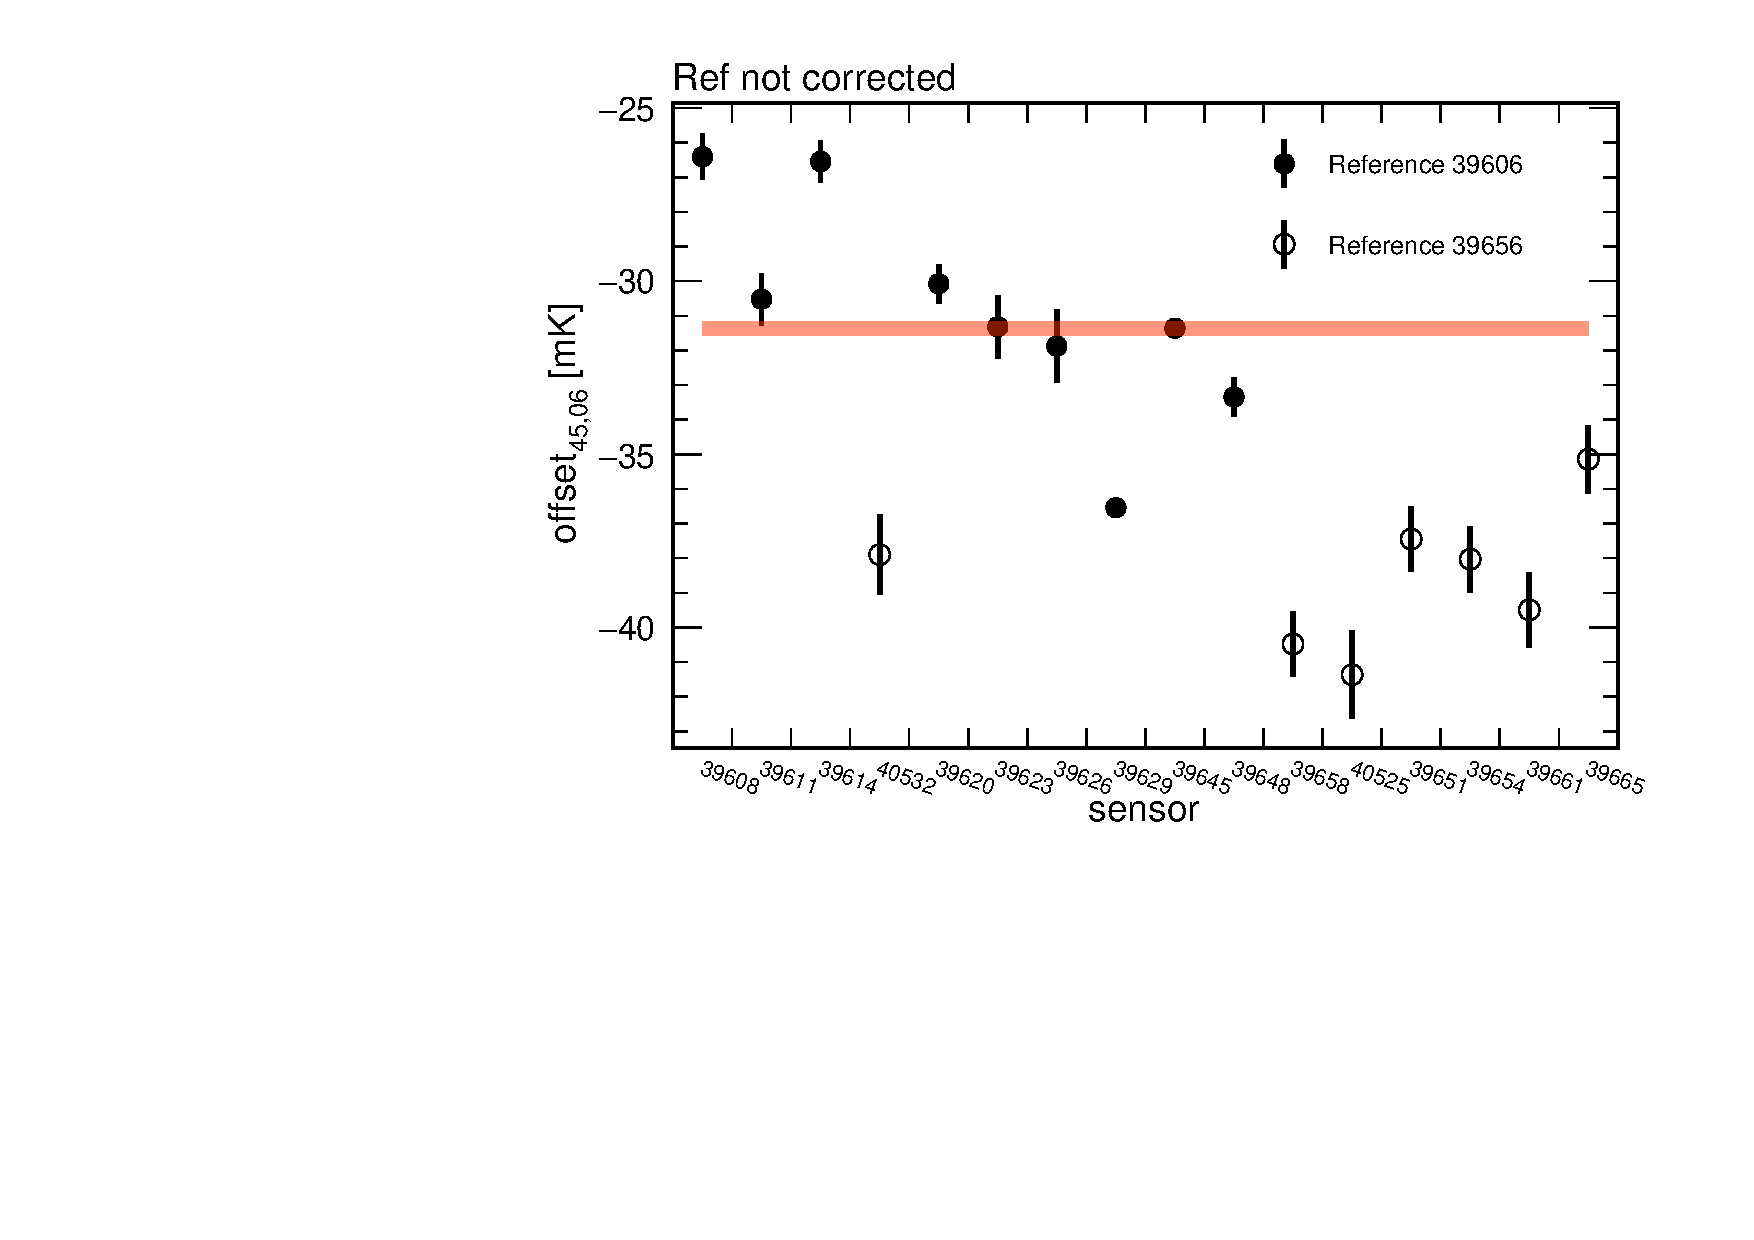
\includegraphics[width=0.49\textwidth]{images/figure_15_b.pdf}}
{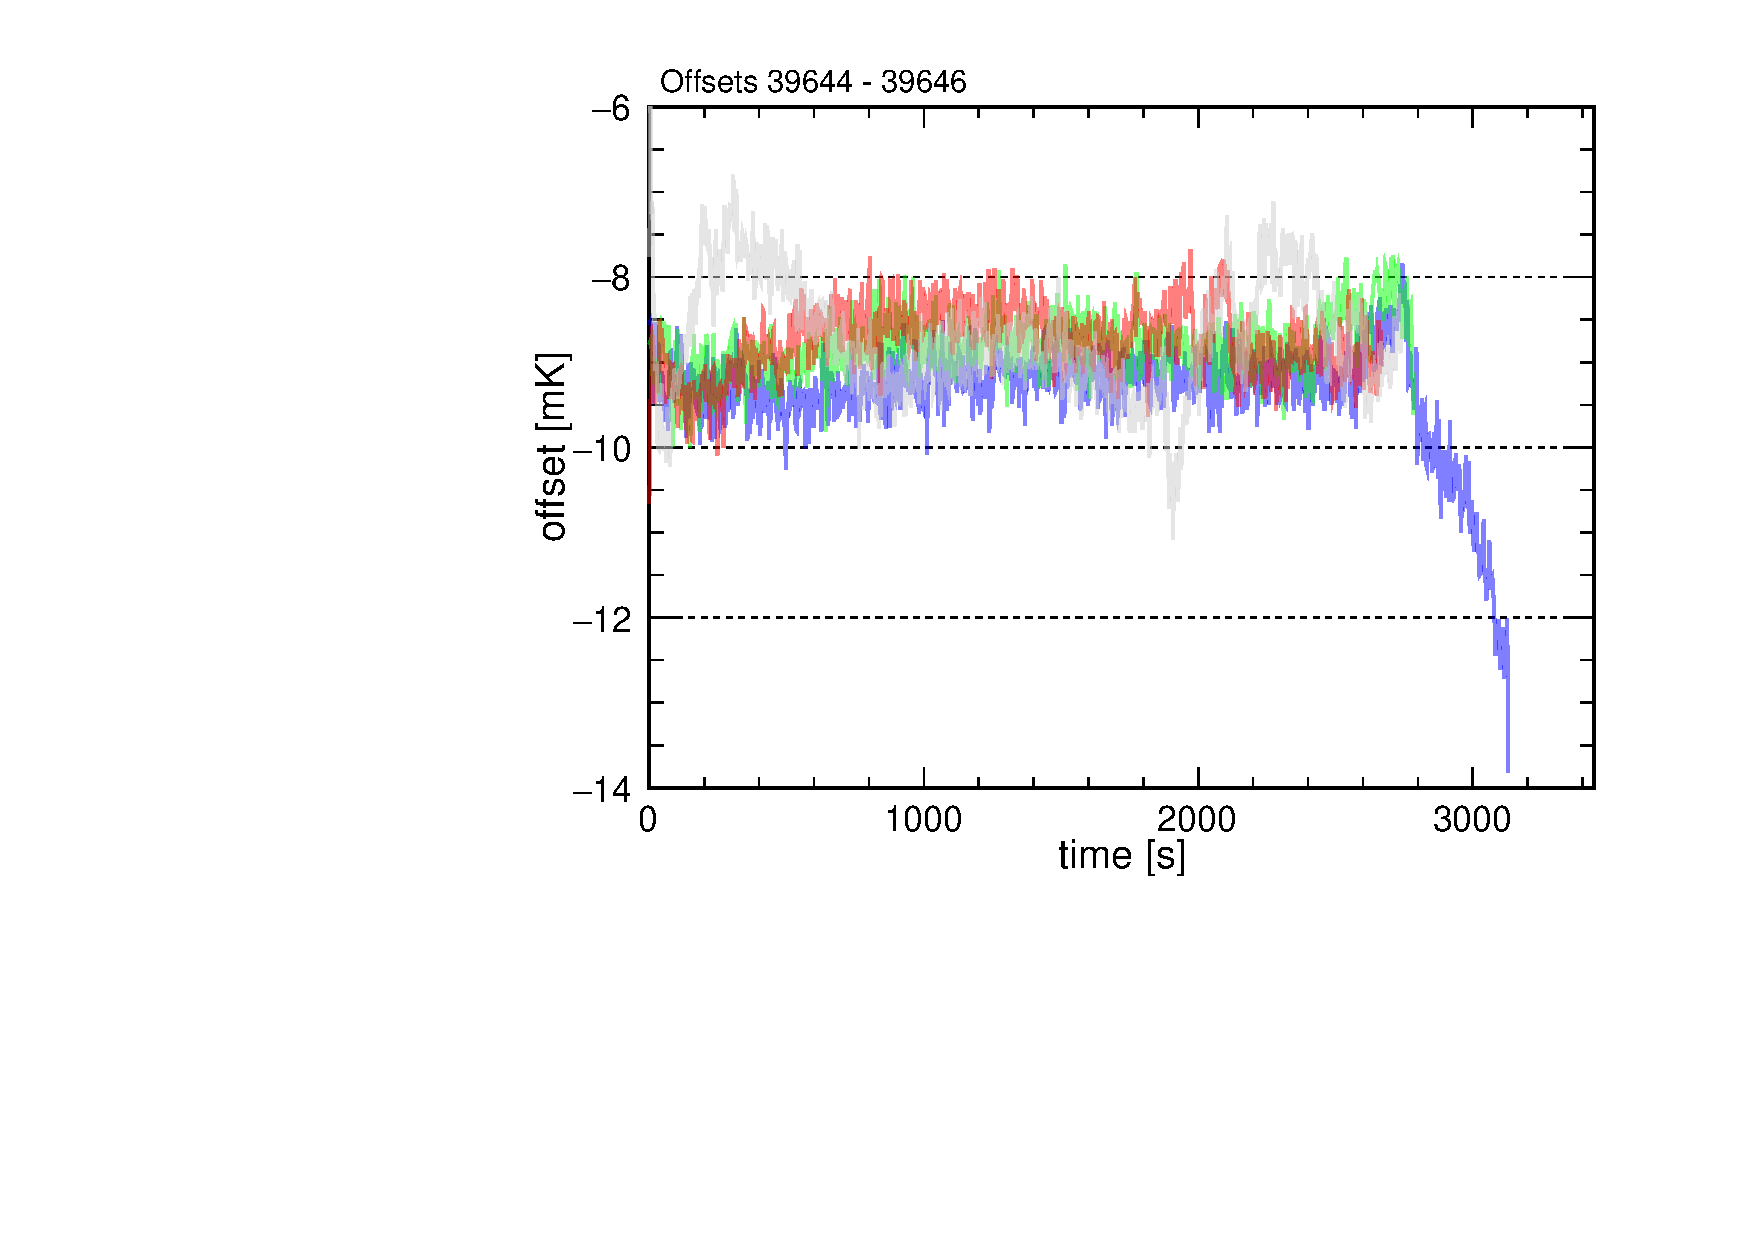
\includegraphics[width=0.49\textwidth]{images/figure_15_a.pdf}}
\caption{$\Delta T_{45,06}$ computed through all sensors of the second round of the calibration procedure. Left: not applying corrections. Right: applying corrections. A clear improvement is obtained using the corrections on the reference sensor. The red line represents the expected value of this calibration constant.}
\label{fig:crosscheck}
\end{figure}